\documentclass[10pt, a4paper]{article}
\usepackage[slantfont, boldfont]{xeCJK}
\usepackage{ulem}
\usepackage{amsmath}
\usepackage{booktabs}
\usepackage{colortbl}
\usepackage[top = 1.0in, bottom = 1.0in, left = 1.0in, right = 1.0in]{geometry}
\usepackage{lipsum}
\usepackage{graphicx}
\usepackage{hyperref}
\usepackage{listings}
\usepackage{xcolor}

\usepackage{circuitikz}
% \usepackage{tikz}
% \usetikzlibrary{circuits.logic.US}


%\setCJKmainfont{SimSun}
%\setCJKmonofont{SimSun}

%\setmainfont[BoldFont={SimHei},ItalicFont={KaiTi}]{SimSun}
%\setsansfont[BoldFont=SimHei]{KaiTi}
%\setmonofont{NSimSun}

\setlength{\parskip}{0.5\baselineskip}
\setlength{\parindent}{2em}

\newcolumntype{Y}{>{\columncolor{red}}p{12pt}}
\newcolumntype{N}{>{\columncolor{white}}p{12pt}}
% \title{???}
% \author{???}


% \lstset{numbers=left,
% numberstyle=\tiny,
% keywordstyle=\color{blue!70}, commentstyle=\color{red!50!green!50!blue!50},
% frame=shadowbox,
% rulesepcolor=\color{red!20!green!20!blue!20}
% }

\lstset{
  % language=[ANSI]c,
  basicstyle=\small,
  numbers=left,
  keywordstyle=\color{blue},
  numberstyle={\tiny\color{lightgray}},
  stepnumber=1, %行号会逐行往上递增
  numbersep=5pt,
  commentstyle=\small\color{red},
  backgroundcolor=\color[rgb]{0.95,1.0,1.0},
  showspaces=false,
  showtabs=false,
  frame=shadowbox, framexleftmargin=5mm, rulesepcolor=\color{red!20!green!20!blue!20!},
% frame=single,
%  TABframe=single,
  tabsize=4,
  breaklines=tr,
  extendedchars=false %这一条命令可以解决代码跨页时,章节标题,页眉等汉字不显示的问题
}
			
\newcommand{\fullimage}[1]{
	\begin{flushleft}
		\includegraphics[width=\textwidth]{#1}
	\end{flushleft}
}
			
\newcommand{\centerimage}[1]{
	\begin{center}
		\includegraphics{#1}
	\end{center}
}

\newcommand{\pause}[0]{}


\title{Homework 3}
\author{计52 宋世虹 2015011267}
\date{2017年6月}

\begin{document}

	\maketitle

  \section{对象与函数}
  对象:

    \begin{itemize}
      \item Node:表示seam dp时每一个点的权值和路径中上一个点的值。
      \item type:表示当前要carve的是列还是行。
      \item newPoint:表示cut完的seam中的一个点。
      \item T:双向缩放的时候所用的数据结构,其中存有:当前图片,seam掉一行或一列后的图片,seam掉一行的路径,seam掉一列的路径,seam掉一行的cost,seam掉一列的cost,上一次choose了seam掉一行还是一列,当前的图片的seam权值。
    \end{itemize}

    函数:

    \begin{itemize}
      \item inImage:判断一个点是否在图片内。
      \item calculateEnergy:计算论文中所述能量,可以用不同算子。
      \item DP:通过energy函数计算seam,dp出全图每点的权值,存在seam中。
      \item calculateMin:根据seam图计算最小的seam,返回最小的那一列(行)标。
      \item removeline:根据已得的seam移去一行或一列。
      \item addLine:根据已得的seam重新在删去seam的图中加上一条红色的seam。
      \item getInfo:对于一个已知图片的T,计算它的行列seam。
      \item onMouse:将鼠标选中的区域染红。
    \end{itemize}
  \section{seam的求解}
    使用上述calculate energy和dp函数即可。

    代码:

    \begin{lstlisting}
void calculateEnergy(Mat& image,double** energy,int row,int col)
{
  Mat imageXY8UC = image.clone();    
  Mat imageX=Mat::zeros(image.size(),CV_8UC3);  
    Mat imageY=Mat::zeros(image.size(),CV_8UC3);     
    Mat imageXY=Mat::zeros(image.size(),CV_8UC3);    
    Mat imageX8UC;  
    Mat imageY8UC;  
 //    for(int i=0;i<image.rows;i++)  
 //    {  
 //        for(int j=0;j<image.cols;j++)  
 //        {  
 //            //通过指针遍历图像上每一个像素  
 //            for (int k = 0;k < 3;++k)
  //             {
  //              imageX.at<Vec3b>(i,j)[k] =jueduizhi(
  //          (i > 0 && j < image.cols-1 ? image.at<Vec3b>(i-1,j+1)[k] : 0)
  //          + (j < image.cols-1 ? image.at<Vec3b>(i,j+1)[k]*2 : 0)
  //          + (i < image.rows-1 && j < image.cols-1 ? image.at<Vec3b>(i+1,j+1)[k] : 0)
  //          - (i > 0 && j > 0 ? image.at<Vec3b>(i-1,j-1)[k] : 0)
  //          - (j > 0 ? image.at<Vec3b>(i,j-1)[k]*2 : 0)
  //          - (i < image.rows-1 && j > 0 ? image.at<Vec3b>(i+1,j-1)[k] : 0)
  //        );  
  //              imageY.at<Vec3b>(i,j)[k]=jueduizhi(
  //          (i < image.rows-1 && j > 0 ? image.at<Vec3b>(i+1,j-1)[k] : 0)
  //          + (i < image.rows-1 ? image.at<Vec3b>(i+1,j)[k]*2 : 0)
  //          + (i < image.rows-1 && j < image.cols-1 ? image.at<Vec3b>(i+1,j+1)[k] : 0)
  //          - (i > 0 && j > 0 ? image.at<Vec3b>(i-1,j-1)[k] : 0)
  //          - (i > 0 ? image.at<Vec3b>(i-1,j)[k]*2 : 0)
  //          - (i > 0 && j < image.cols-1 ? image.at<Vec3b>(i-1,j+1)[k] : 0)
  //        );  
  //          }
 //        }  
 //    }  
 //    addWeighted(imageX,0.5,imageY,0.5,0,imageXY);//融合X、Y方向    
 //    convertScaleAbs(imageX,imageX8UC);  
 //    convertScaleAbs(imageY,imageY8UC);  
 //    convertScaleAbs(imageXY,imageXY8UC);   //转换为8bit图像  
        for(int i=0;i<image.rows;i++)  
      {  
          for(int j=0;j<image.cols;j++)  
          {  
              //通过指针遍历图像上每一个像素  
              for (int k = 0;k < 3;++k)
                {
                  imageXY8UC.at<Vec3b>(i,j)[k] =jueduizhi(
              - (i > 0 ? image.at<Vec3b>(i-1,j)[k] : 0)
              - (i < image.rows-1 ? image.at<Vec3b>(i+1,j)[k]*2 : 0)
              - (j < image.cols-1 ? image.at<Vec3b>(i,j+1)[k] : 0)
              - (j > 0 ? image.at<Vec3b>(i,j-1)[k] : 0)
              + (image.at<Vec3b>(i,j)[k]*4)
            );  
              }
          }  
        }
  for (int i = 0;i < row;++i)
  {
    for (int j = 0;j < col;++j)
    {
      energy[i][j] = 0;
      for (int k = 0;k < 3;++k)
      {
        energy[i][j] += (int)(imageXY8UC.at<cv::Vec3b>(i,j)[k]);
      }
      // energy[i][j] += (int)(imageXY8UC.at<uchar>(i,j));
    }
  }
}
    \end{lstlisting}
	   calculatEnergy用了不同的算子,会在后文中提到,energy会用这三通道的输出结果的直接和作为真正的energy。

     DP计算了论文中所给的方法,每次选择上面的左中右三个pixel的seam权值,来得到当前最小的seam权值。在计算的过程中记录seam的路径。
  \section{使用不同算子进行测试}
    笔者使用了Sobel算子和拉普拉斯算子。以下是效果:

    原图:(之后横纵都cut 1$\%$)

    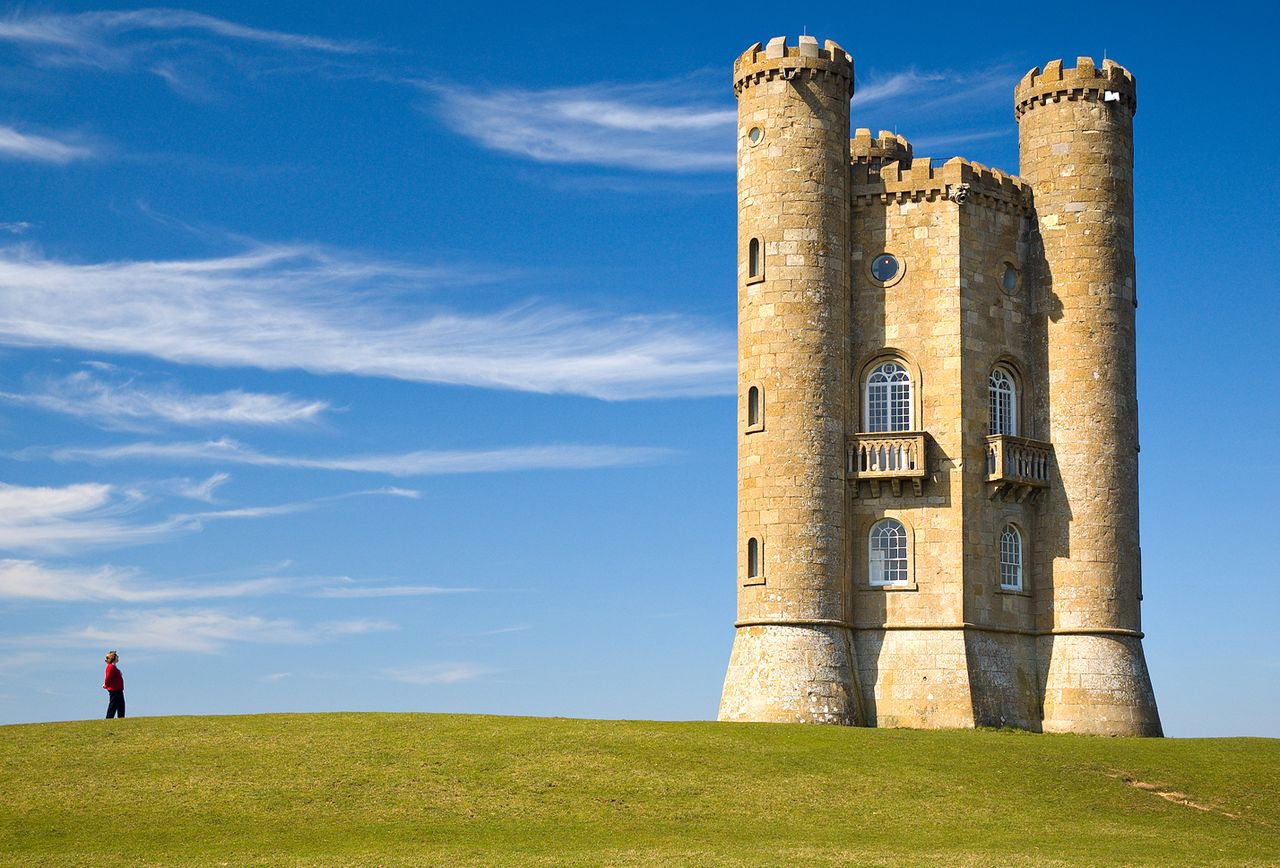
\includegraphics[scale = .3]{1.jpg}

    Laplacian:

    \includegraphics[scale = .3]{1lapseam.png}

    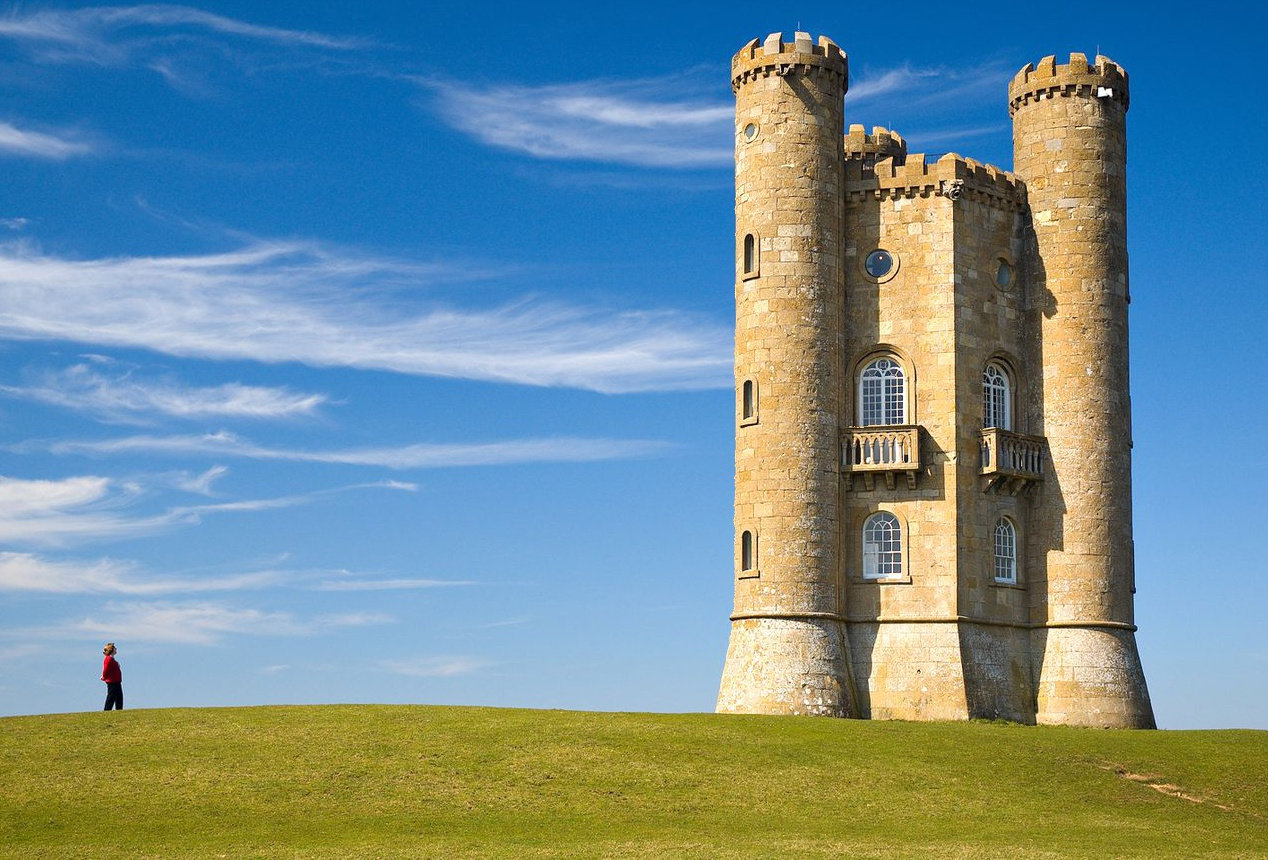
\includegraphics[scale = .3]{1lap.jpg}

    Sobel:

    \includegraphics[scale = .3]{1sobelseam.png}

    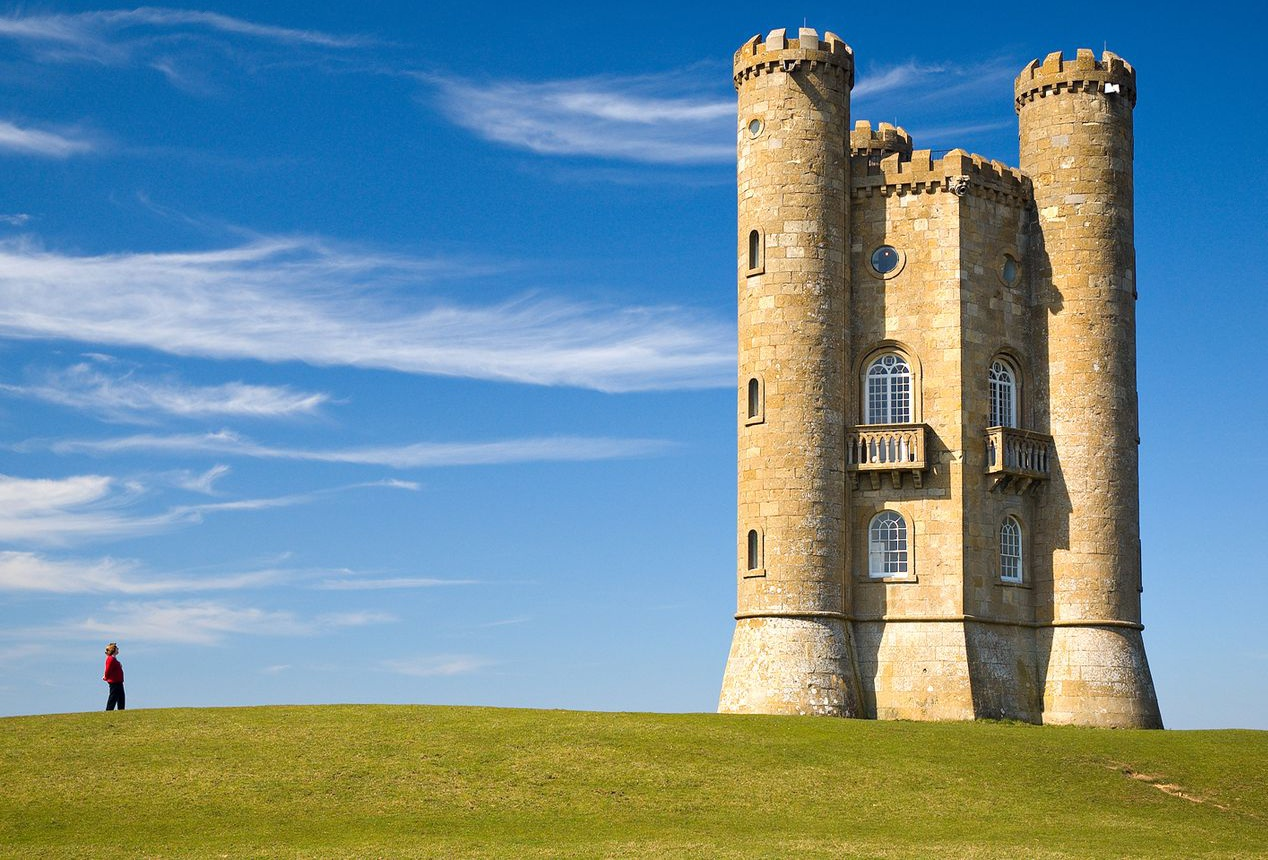
\includegraphics[scale = .3]{1sobel.jpg}

    原图:(之后横纵都cut 1$\%$)

    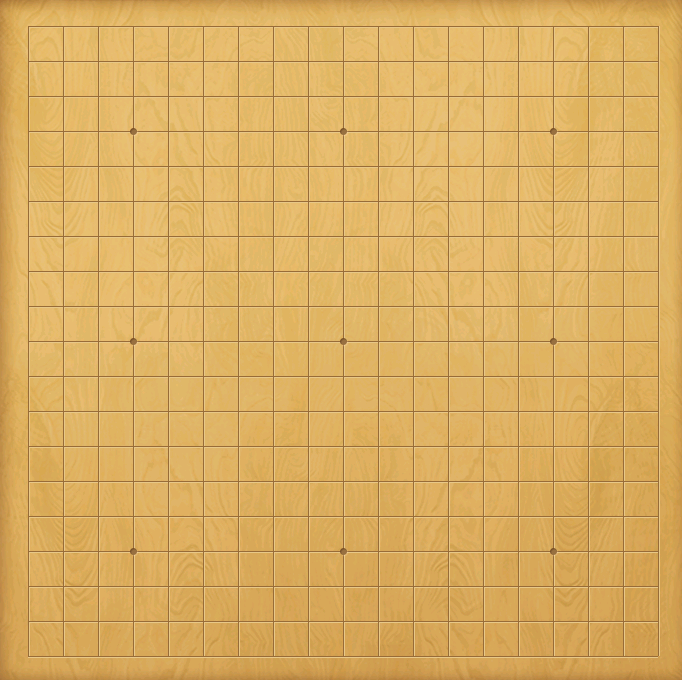
\includegraphics[scale = .2]{2.png}

    Laplacian:

    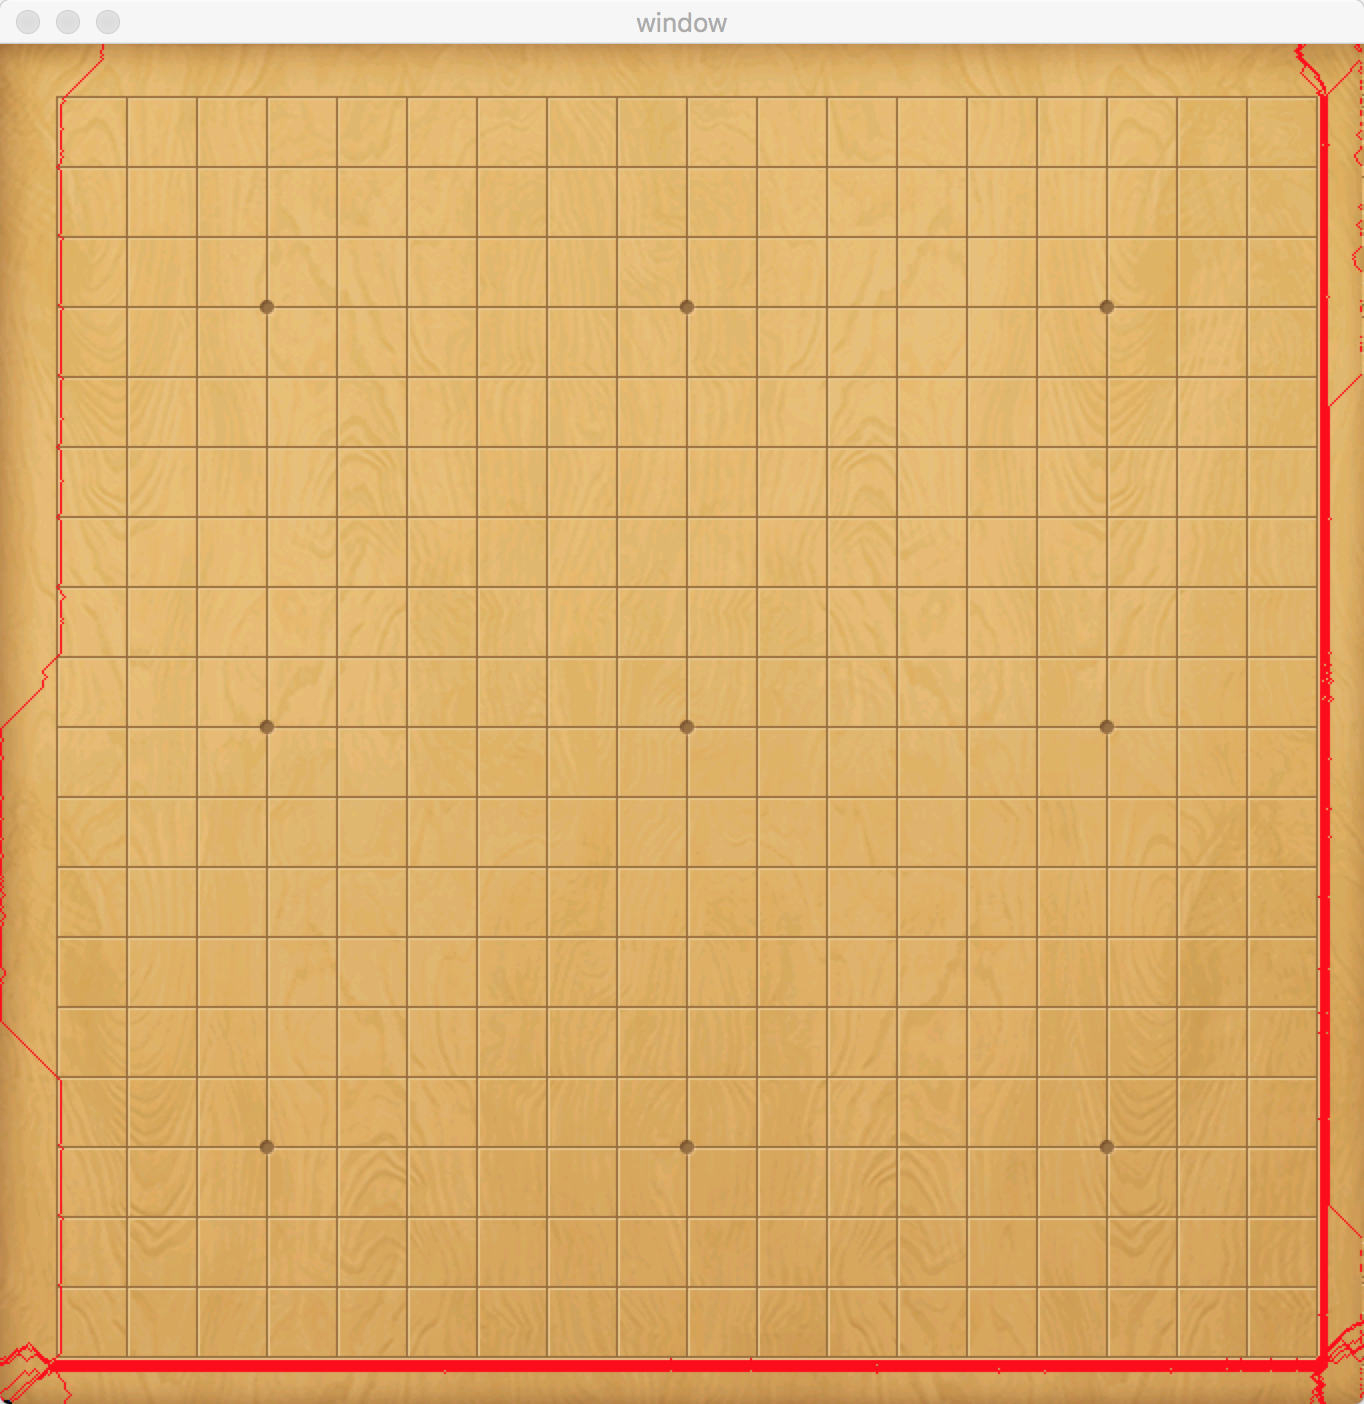
\includegraphics[scale = .1]{2lapseam.png}

    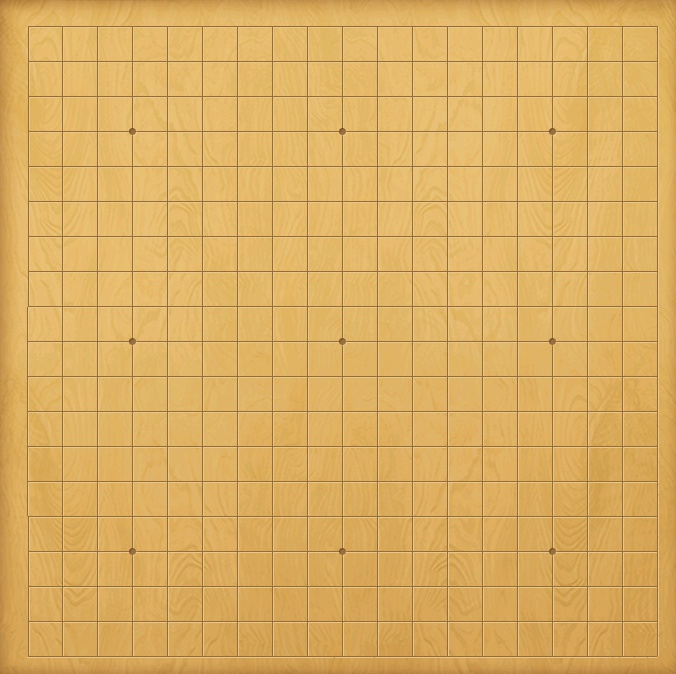
\includegraphics[scale = .3]{2lap.jpg}

    Sobel:

    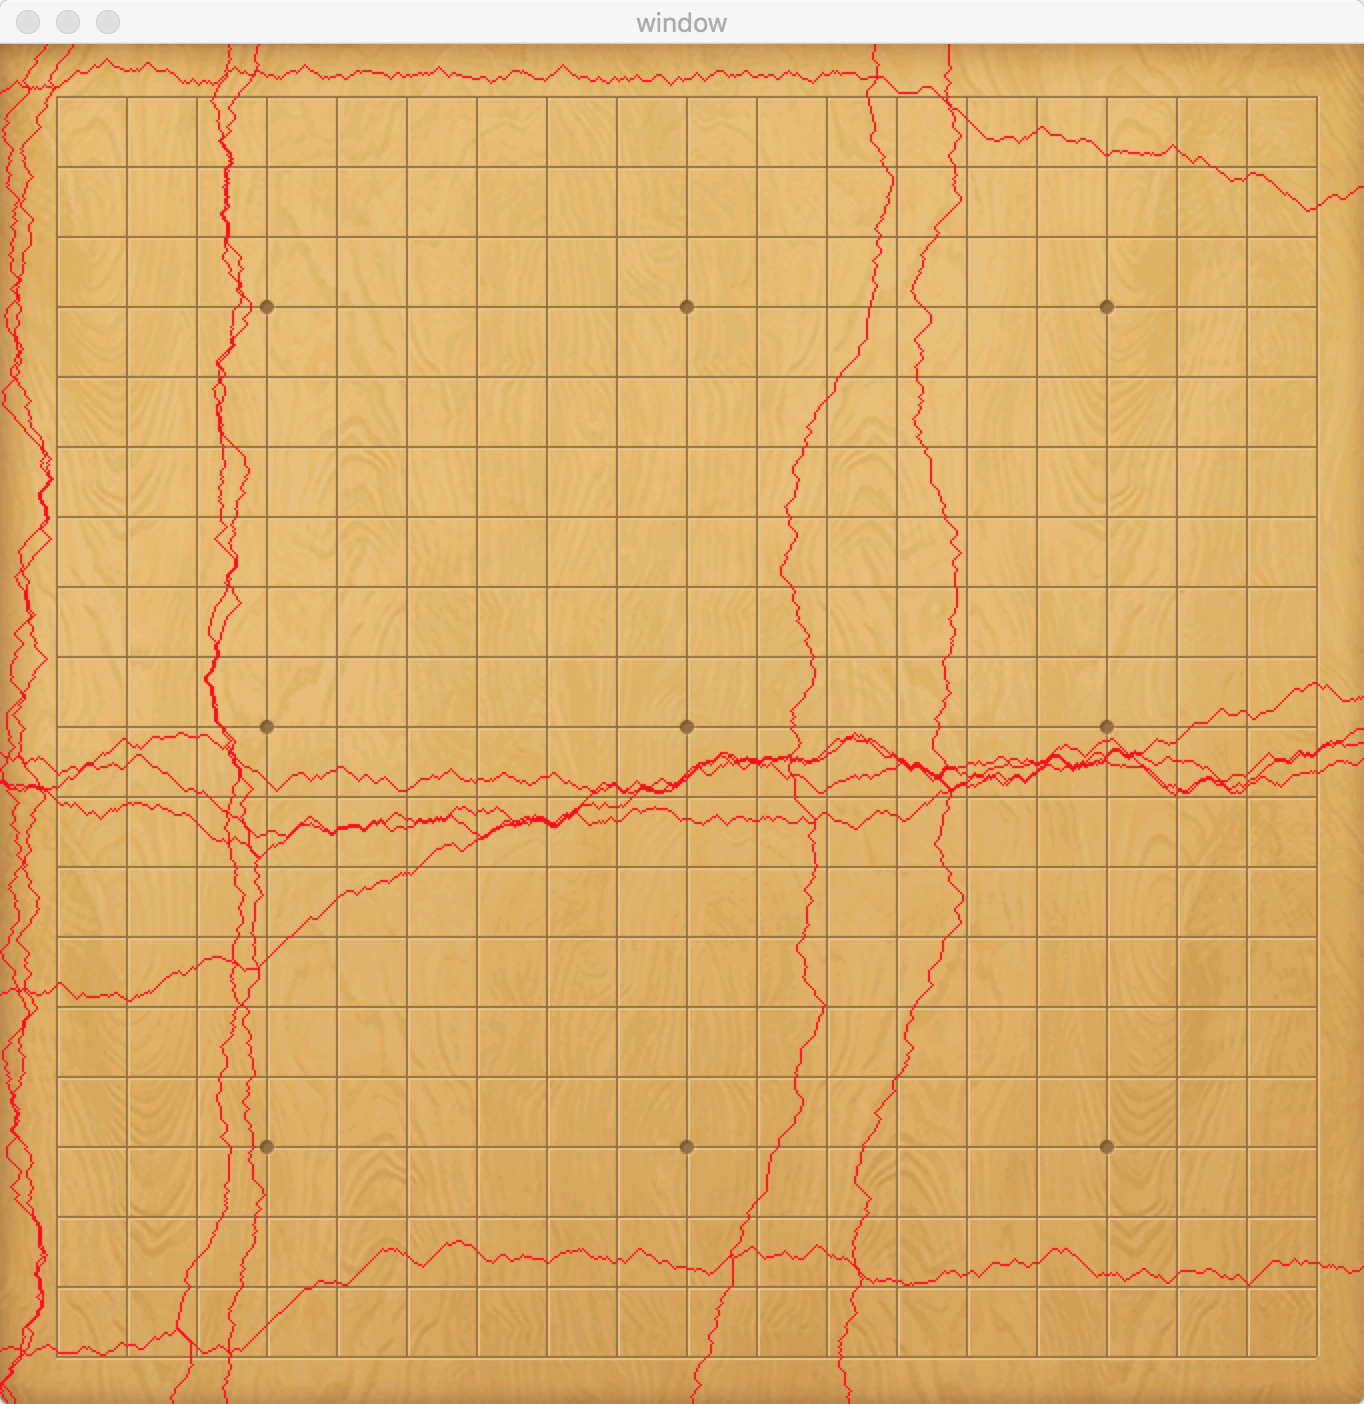
\includegraphics[scale = .1]{2sobelseam.png}

    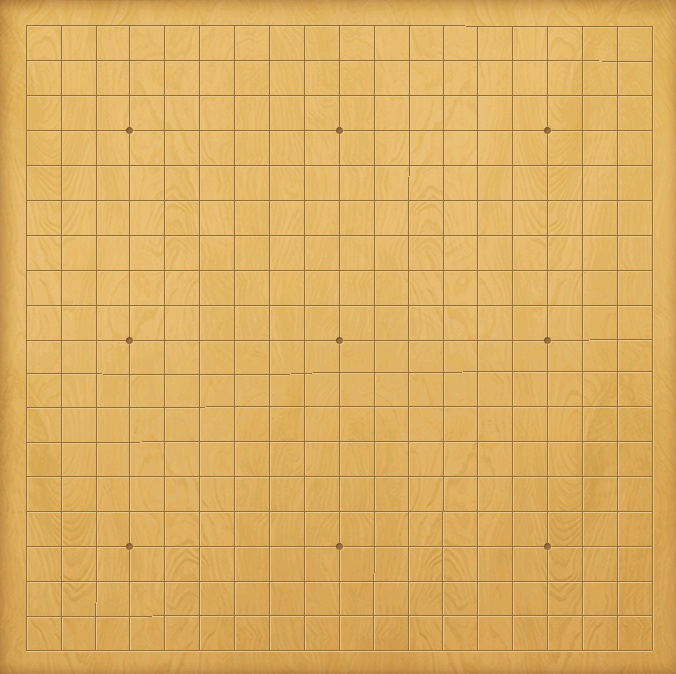
\includegraphics[scale = .3]{2sobel.jpg}

    原图:(之后横纵都cut 10$\%$)

    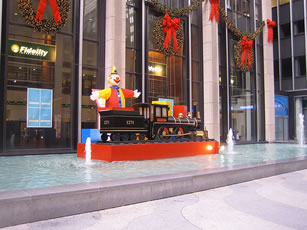
\includegraphics[scale = .3]{3.jpg}

    Laplacian:

    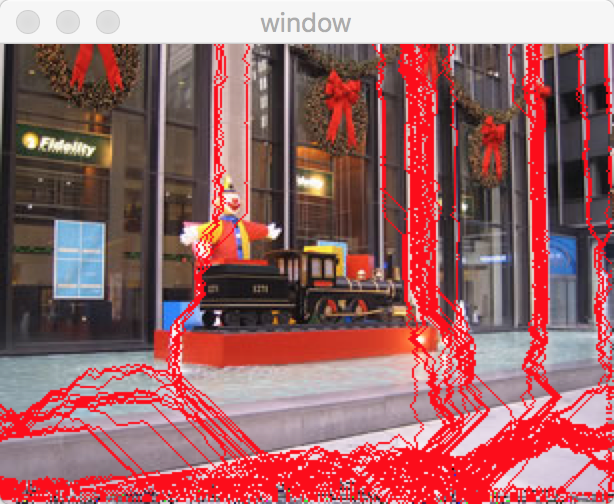
\includegraphics[scale = .3]{3lapseam.png}

    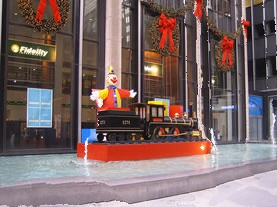
\includegraphics[scale = .3]{3lap.jpg}

    Sobel:

    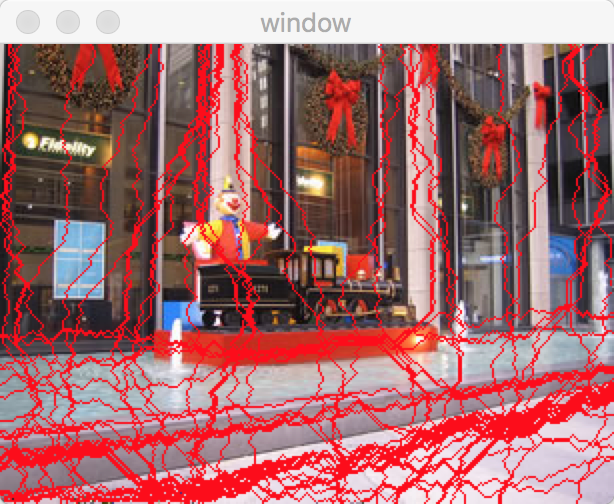
\includegraphics[scale = .3]{3sobelseam.png}

    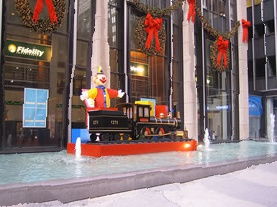
\includegraphics[scale = .3]{3sobel.jpg}

    原图:(之后横纵都cut 10$\%$)

    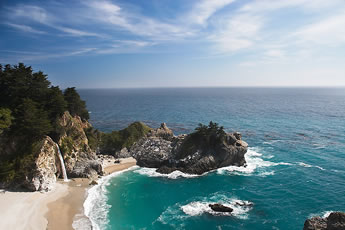
\includegraphics[scale = .3]{4.jpg}

    Laplacian:

    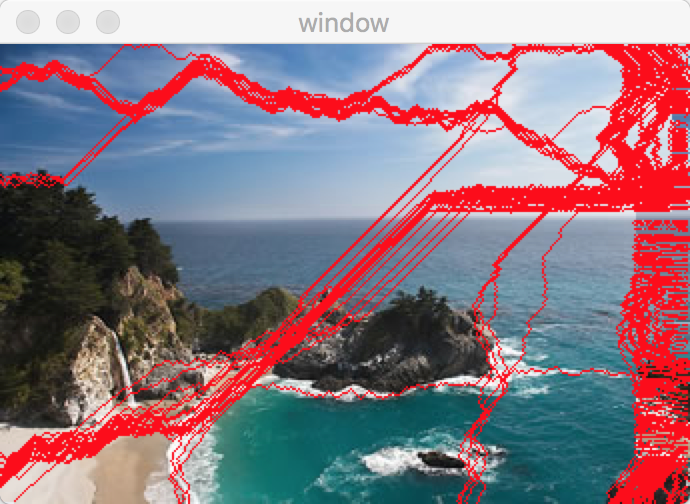
\includegraphics[scale = .3]{4lapseam.png}

    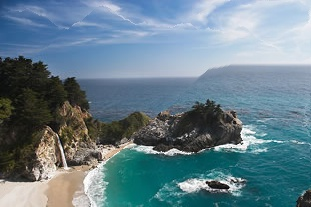
\includegraphics[scale = .3]{4lap.jpg}

    Sobel:

    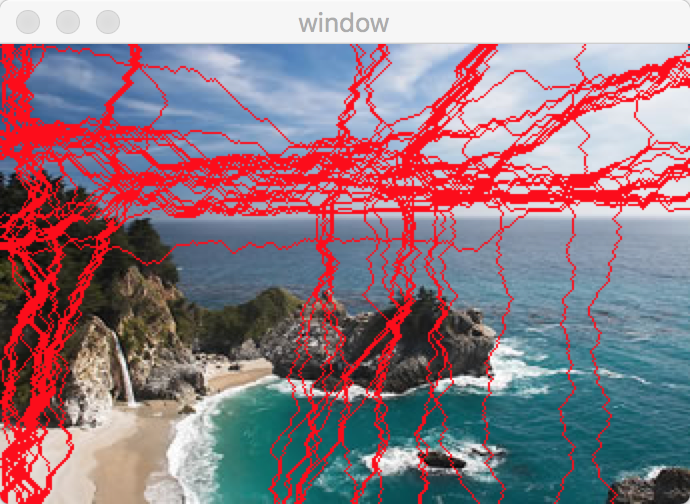
\includegraphics[scale = .3]{4sobelseam.png}

    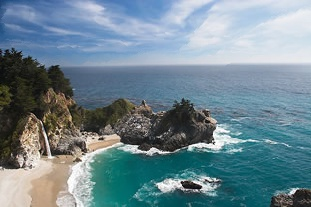
\includegraphics[scale = .3]{4sobel.jpg}

    原图:(之后横纵都cut 1$\%$)

    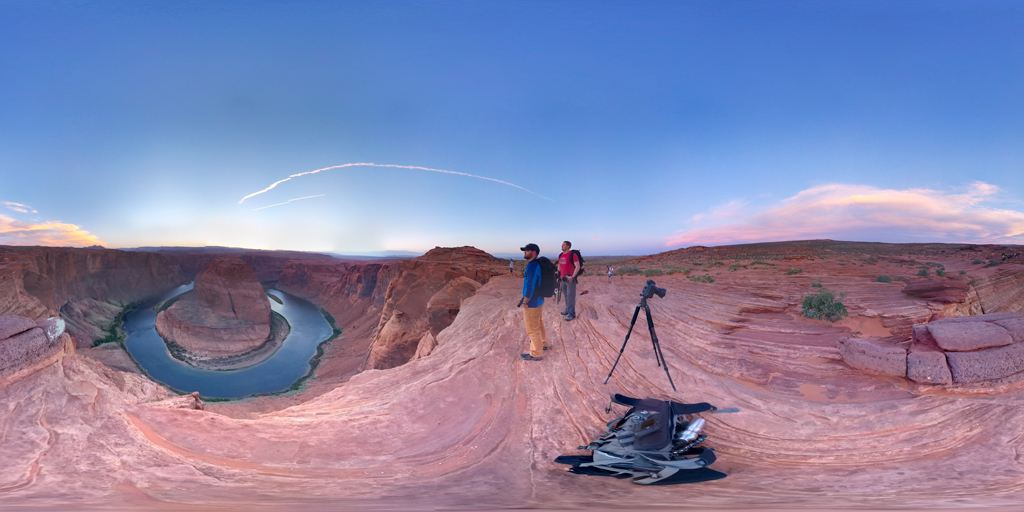
\includegraphics[scale = .3]{5.jpg}

    Laplacian:

    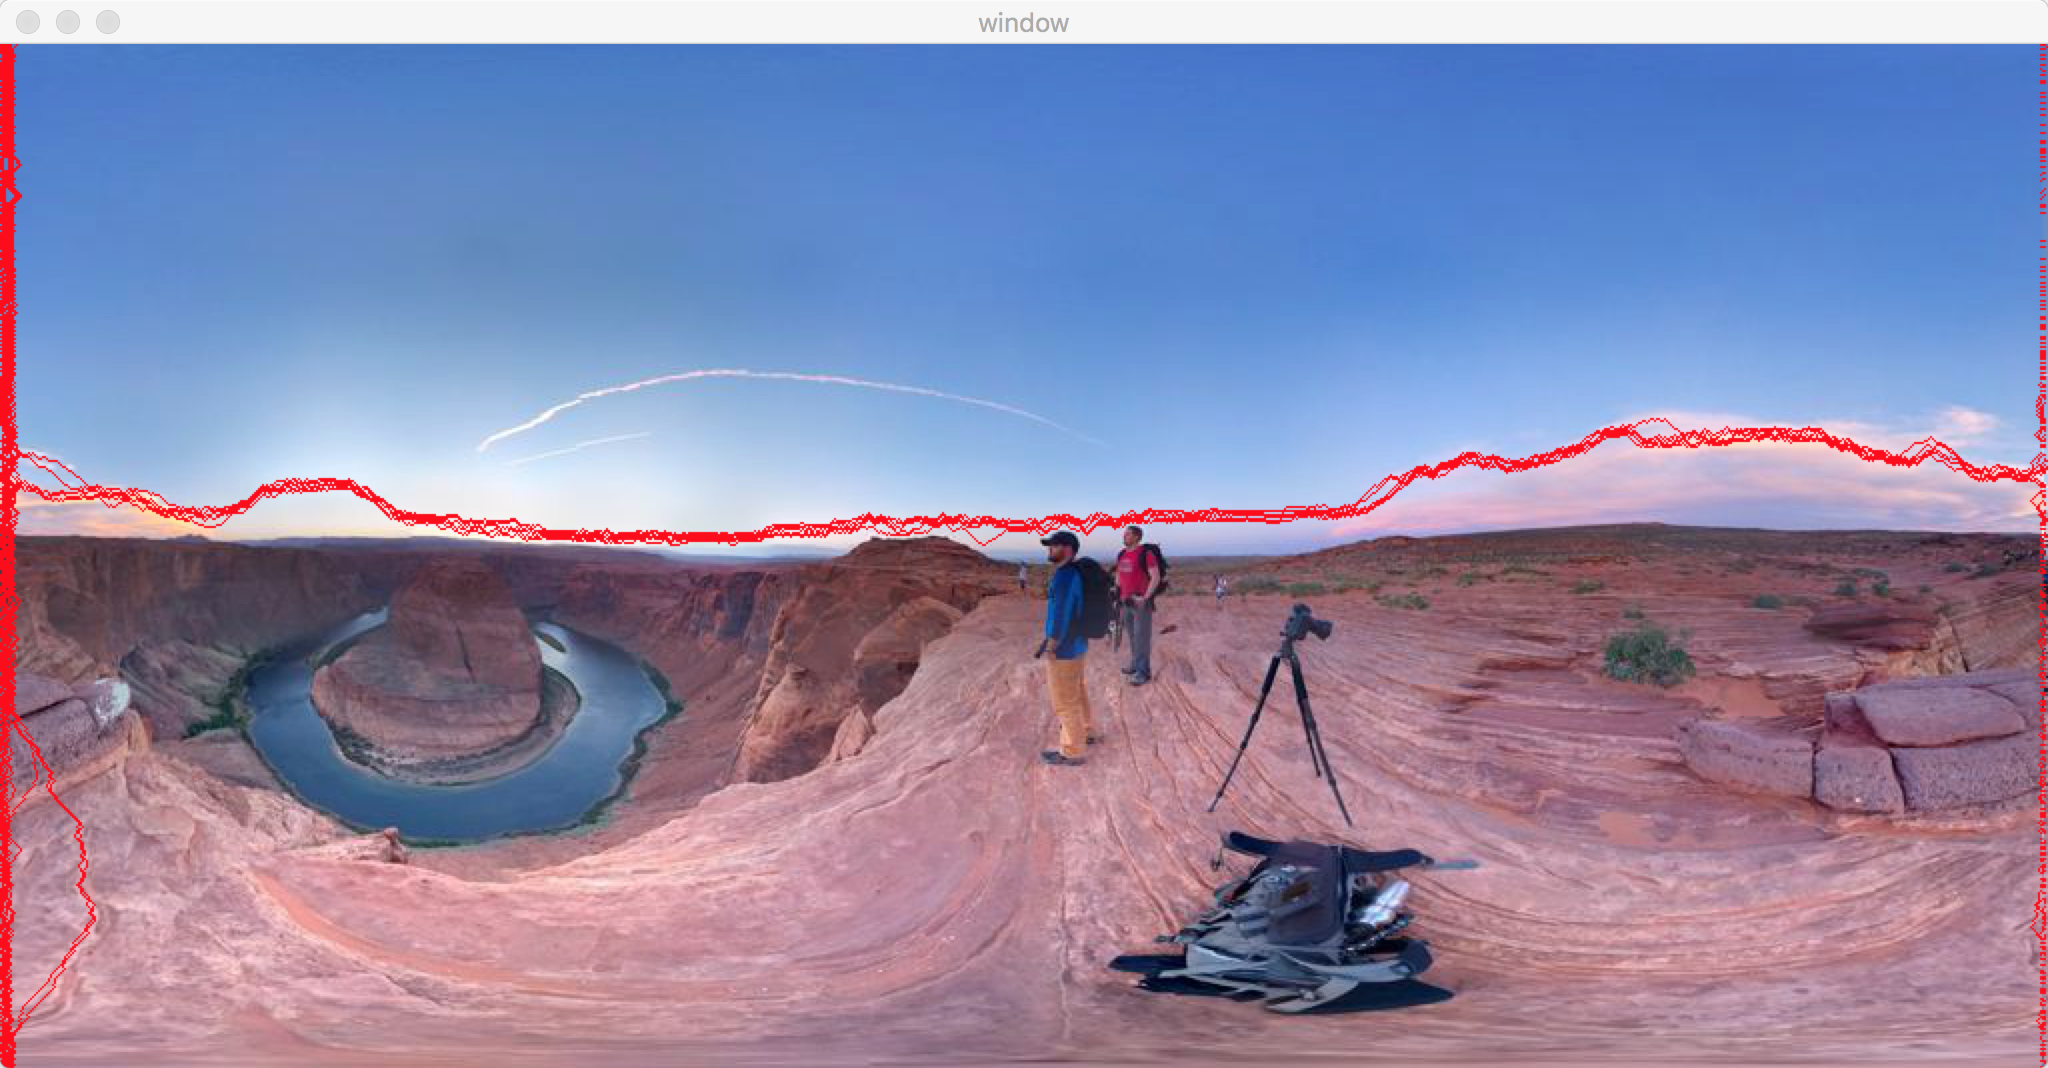
\includegraphics[scale = .3]{5lapseam.png}

    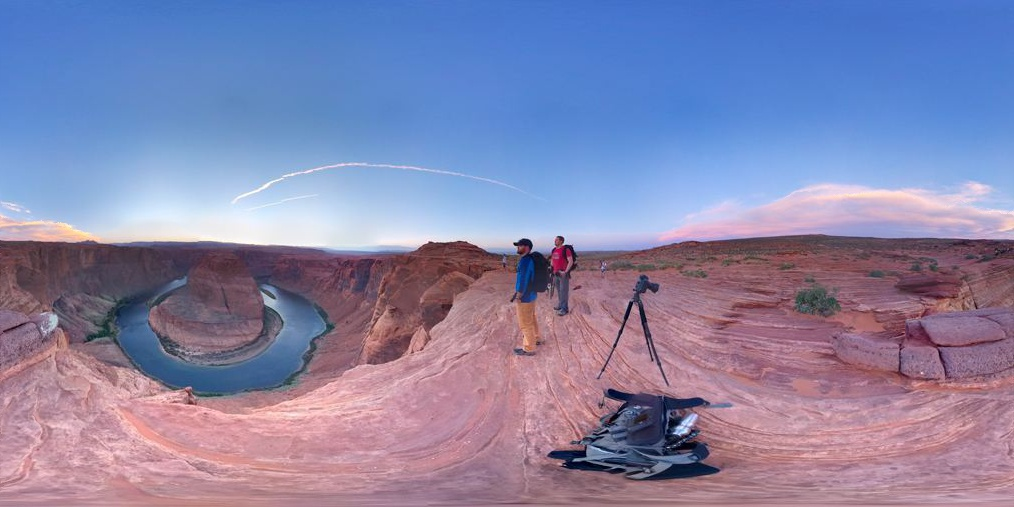
\includegraphics[scale = .3]{5lap.jpg}

    Sobel:

    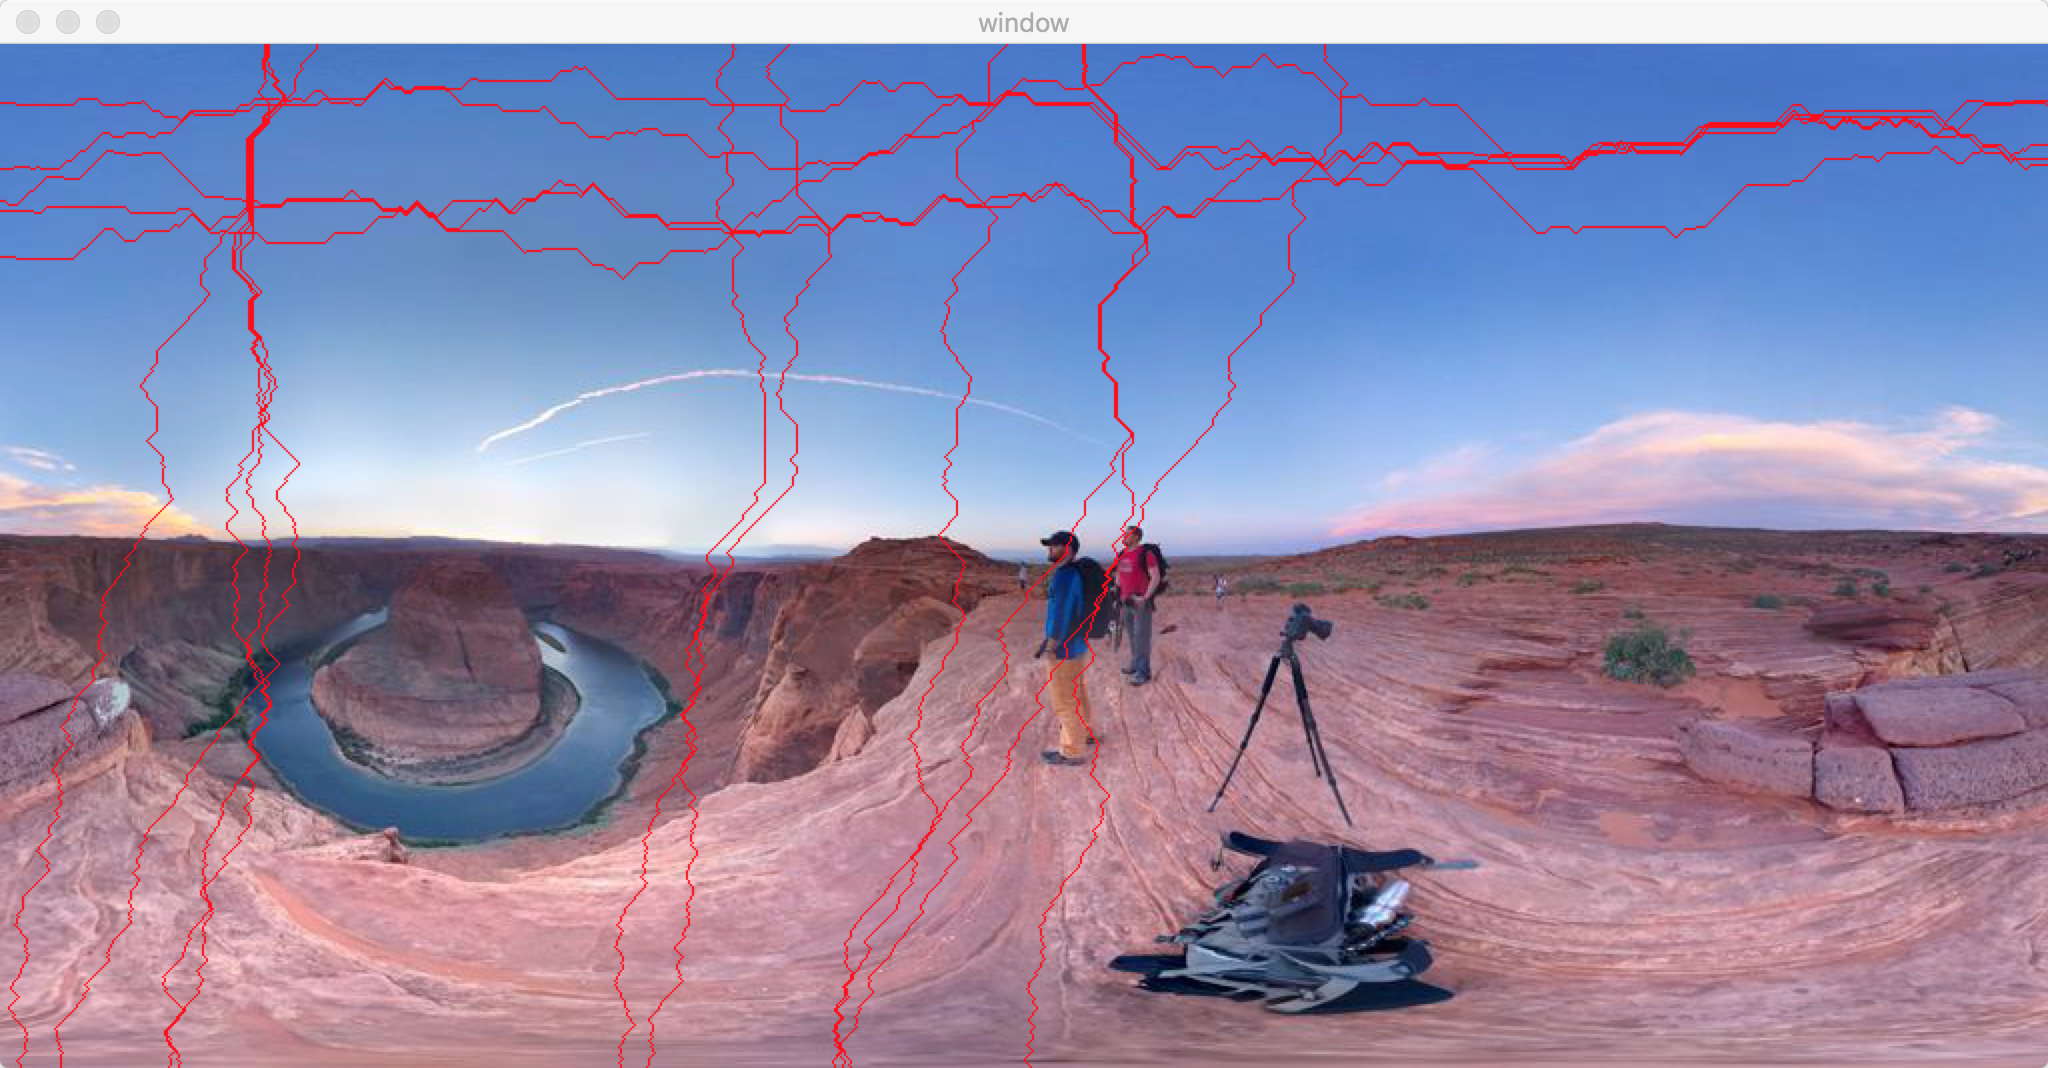
\includegraphics[scale = .3]{5sobelseam.png}

    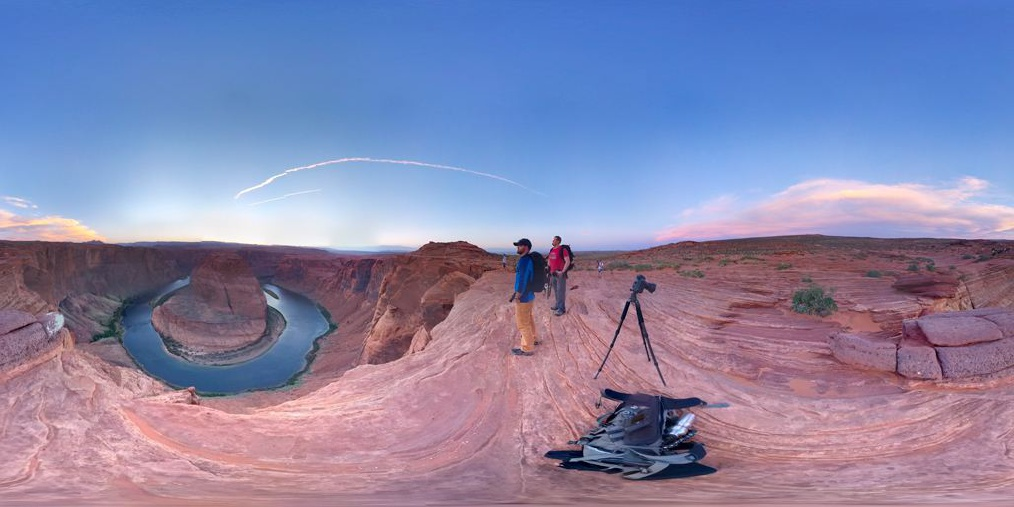
\includegraphics[scale = .3]{5sobel.jpg}

    原图:(之后横纵都cut 0.1$\%$)

    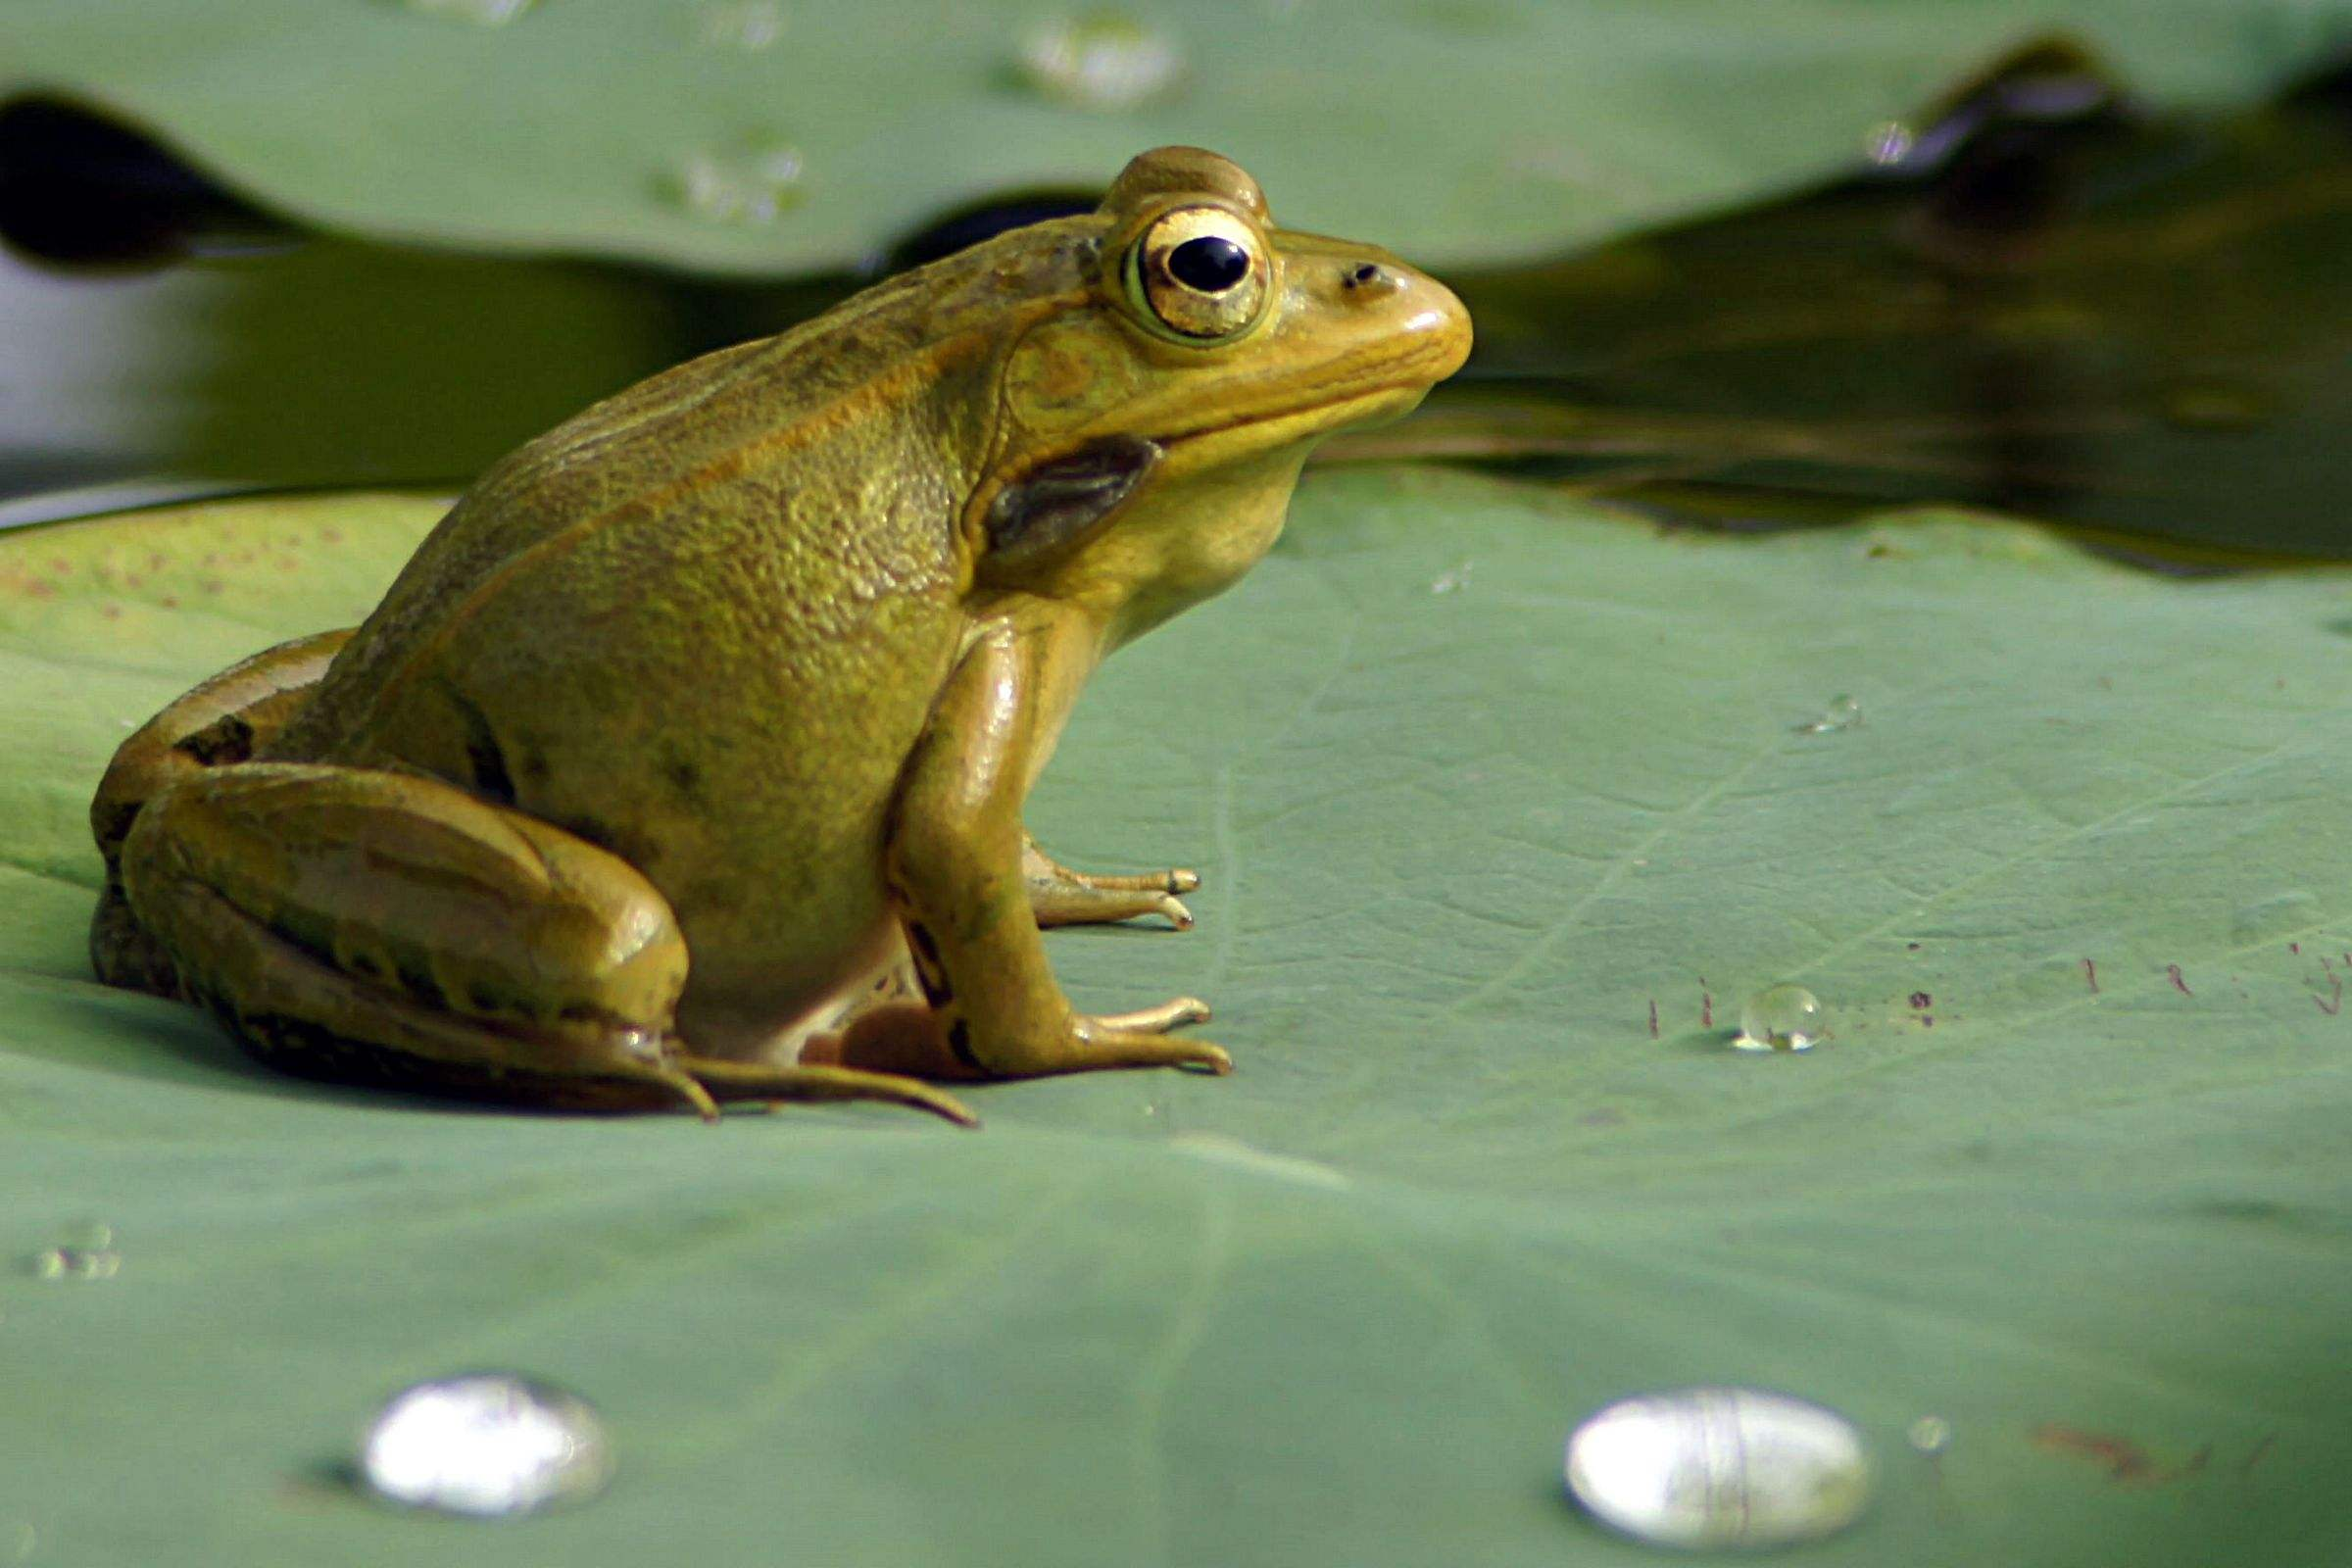
\includegraphics[scale = .1]{6.jpg}

    Laplacian:

    \includegraphics[scale = .1]{6lapseam.png}

    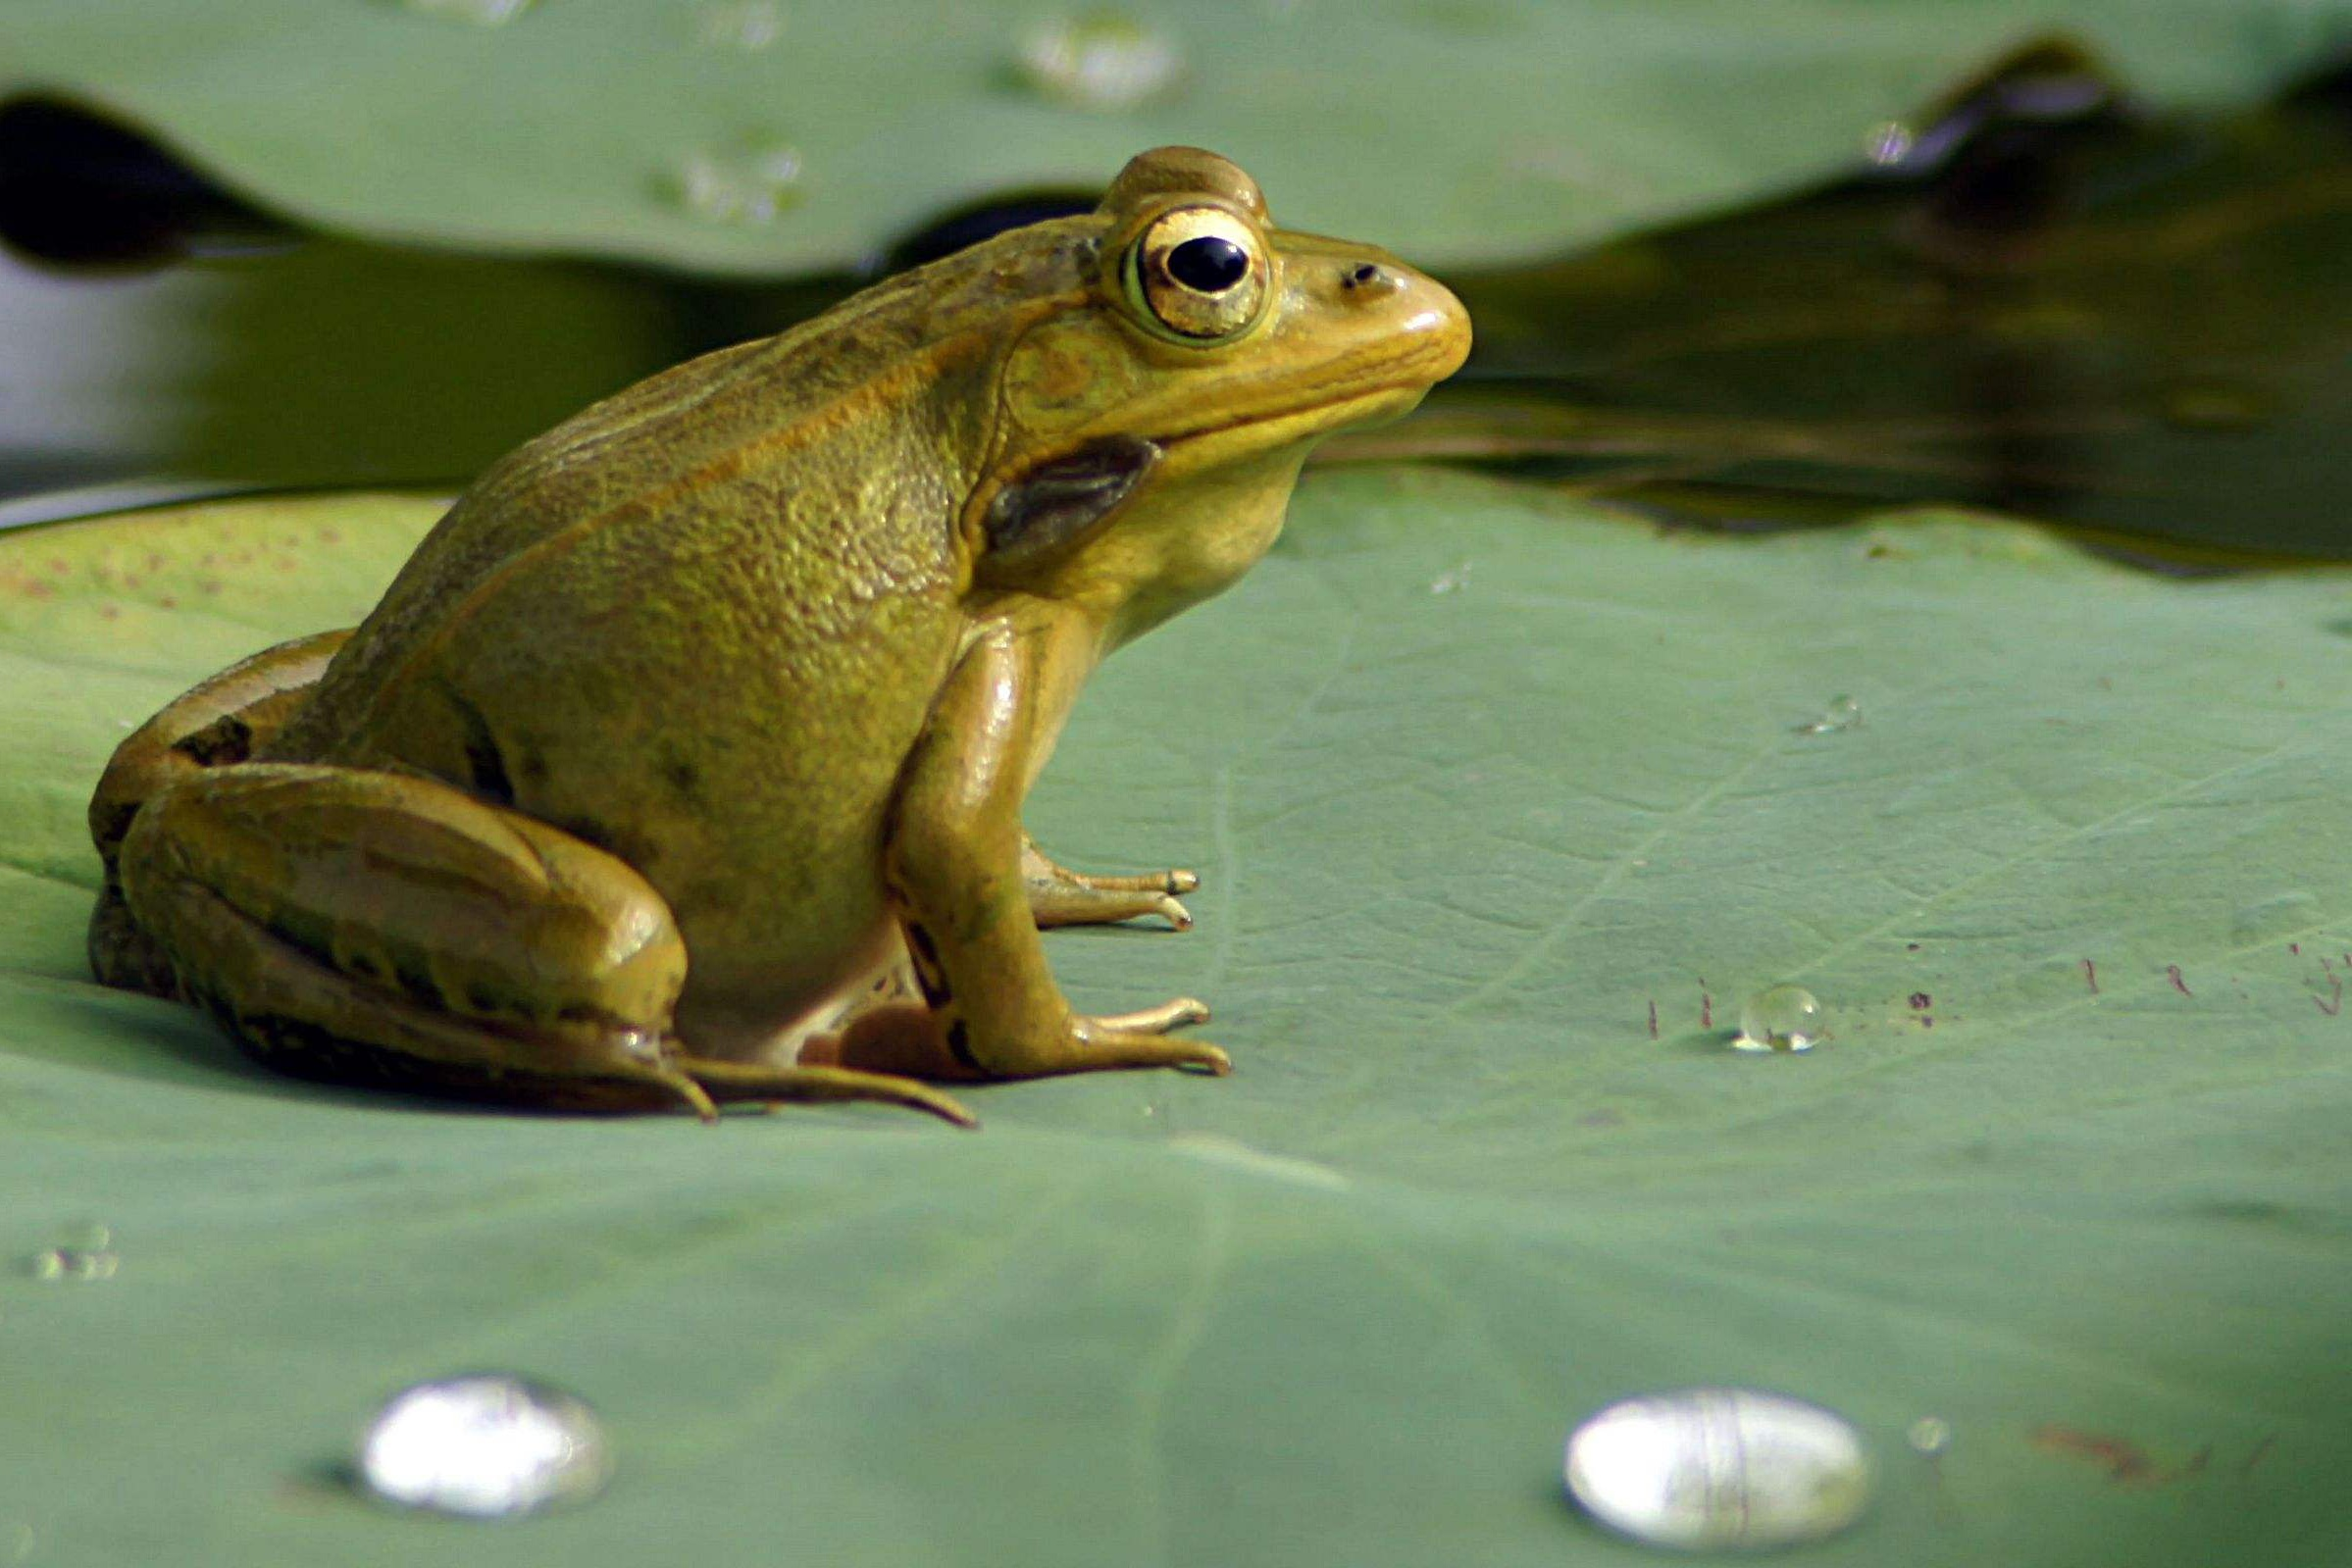
\includegraphics[scale = .1]{6lap.jpg}

    Sobel:

    \includegraphics[scale = .1]{6sobelseam.png}

    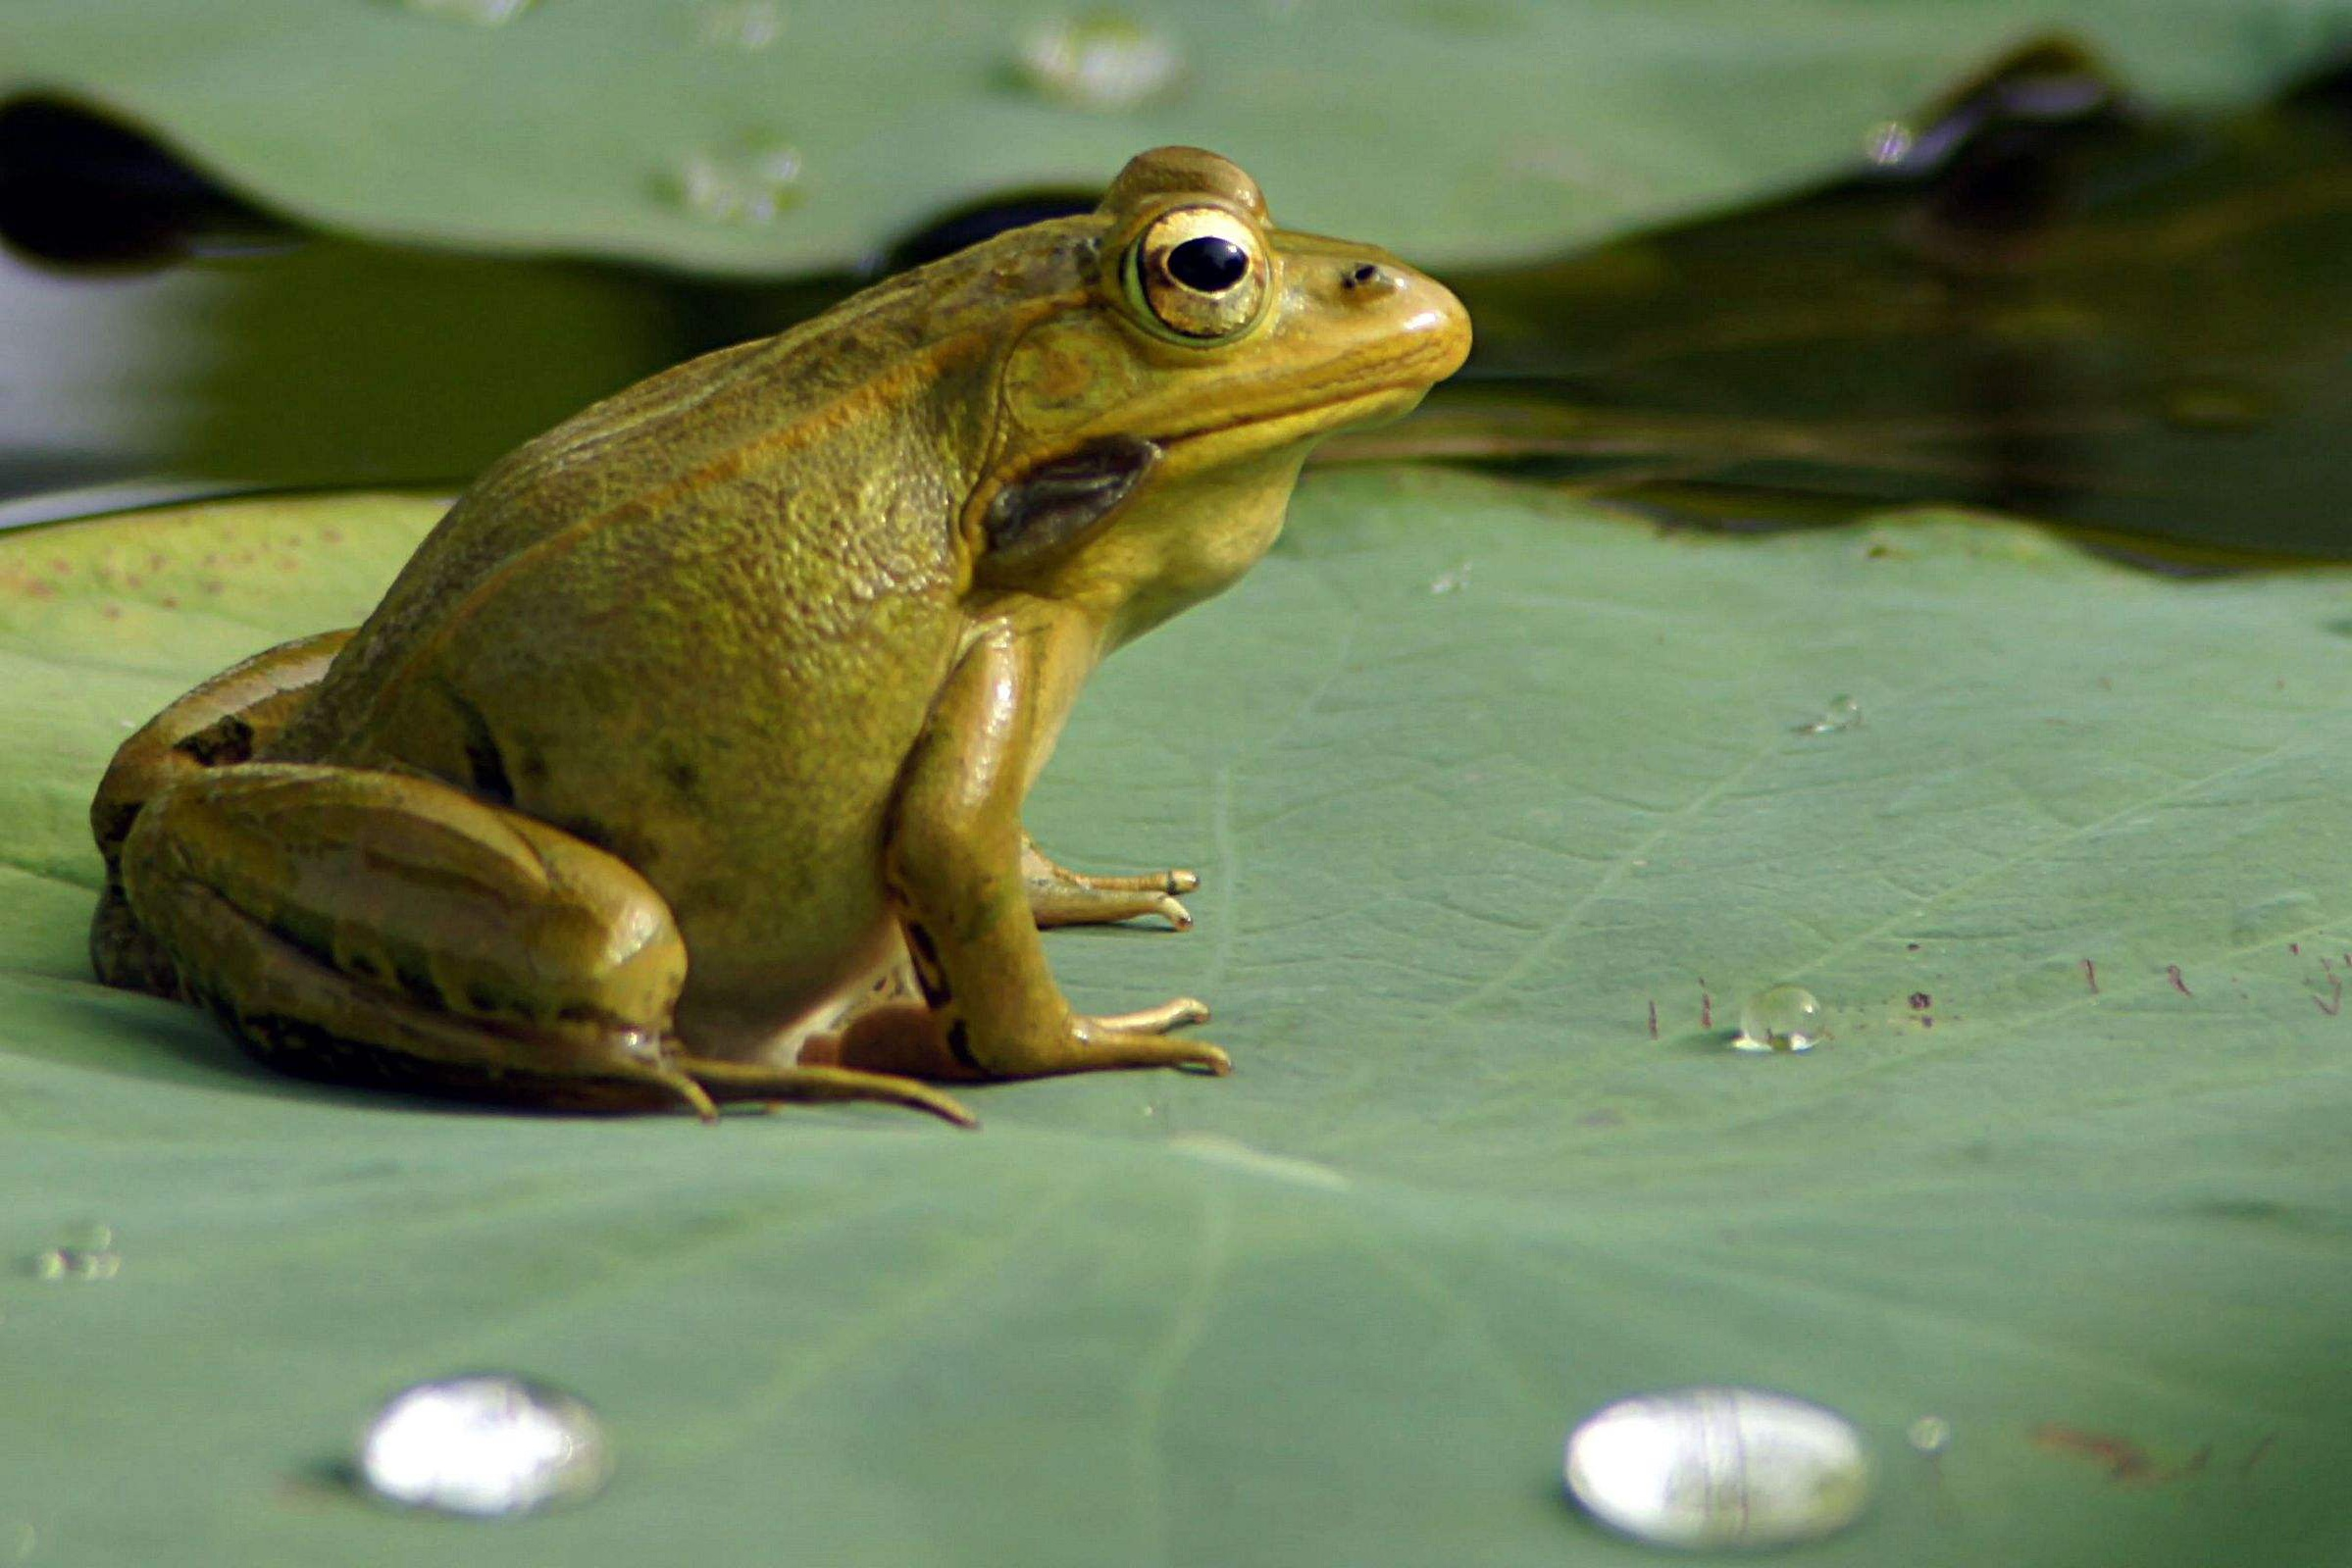
\includegraphics[scale = .1]{6sobel.jpg}
    对应的代码段:
        \begin{lstlisting}
void calculateEnergy(Mat& image,double** energy,int row,int col)
{
  Mat imageXY8UC = image.clone();    
  Mat imageX=Mat::zeros(image.size(),CV_8UC3);  
    Mat imageY=Mat::zeros(image.size(),CV_8UC3);     
    Mat imageXY=Mat::zeros(image.size(),CV_8UC3);    
    Mat imageX8UC;  
    Mat imageY8UC;  
 //    for(int i=0;i<image.rows;i++)  
 //    {  
 //        for(int j=0;j<image.cols;j++)  
 //        {  
 //            //通过指针遍历图像上每一个像素  
 //            for (int k = 0;k < 3;++k)
  //             {
  //              imageX.at<Vec3b>(i,j)[k] =jueduizhi(
  //          (i > 0 && j < image.cols-1 ? image.at<Vec3b>(i-1,j+1)[k] : 0)
  //          + (j < image.cols-1 ? image.at<Vec3b>(i,j+1)[k]*2 : 0)
  //          + (i < image.rows-1 && j < image.cols-1 ? image.at<Vec3b>(i+1,j+1)[k] : 0)
  //          - (i > 0 && j > 0 ? image.at<Vec3b>(i-1,j-1)[k] : 0)
  //          - (j > 0 ? image.at<Vec3b>(i,j-1)[k]*2 : 0)
  //          - (i < image.rows-1 && j > 0 ? image.at<Vec3b>(i+1,j-1)[k] : 0)
  //        );  
  //              imageY.at<Vec3b>(i,j)[k]=jueduizhi(
  //          (i < image.rows-1 && j > 0 ? image.at<Vec3b>(i+1,j-1)[k] : 0)
  //          + (i < image.rows-1 ? image.at<Vec3b>(i+1,j)[k]*2 : 0)
  //          + (i < image.rows-1 && j < image.cols-1 ? image.at<Vec3b>(i+1,j+1)[k] : 0)
  //          - (i > 0 && j > 0 ? image.at<Vec3b>(i-1,j-1)[k] : 0)
  //          - (i > 0 ? image.at<Vec3b>(i-1,j)[k]*2 : 0)
  //          - (i > 0 && j < image.cols-1 ? image.at<Vec3b>(i-1,j+1)[k] : 0)
  //        );  
  //          }
 //        }  
 //    }  
 //    addWeighted(imageX,0.5,imageY,0.5,0,imageXY);//融合X、Y方向    
 //    convertScaleAbs(imageX,imageX8UC);  
 //    convertScaleAbs(imageY,imageY8UC);  
 //    convertScaleAbs(imageXY,imageXY8UC);   //转换为8bit图像  
        for(int i=0;i<image.rows;i++)  
      {  
          for(int j=0;j<image.cols;j++)  
          {  
              //通过指针遍历图像上每一个像素  
              for (int k = 0;k < 3;++k)
                {
                  imageXY8UC.at<Vec3b>(i,j)[k] =jueduizhi(
              - (i > 0 ? image.at<Vec3b>(i-1,j)[k] : 0)
              - (i < image.rows-1 ? image.at<Vec3b>(i+1,j)[k]*2 : 0)
              - (j < image.cols-1 ? image.at<Vec3b>(i,j+1)[k] : 0)
              - (j > 0 ? image.at<Vec3b>(i,j-1)[k] : 0)
              + (image.at<Vec3b>(i,j)[k]*4)
            );  
              }
          }  
        }
  for (int i = 0;i < row;++i)
  {
    for (int j = 0;j < col;++j)
    {
      energy[i][j] = 0;
      for (int k = 0;k < 3;++k)
      {
        energy[i][j] += (int)(imageXY8UC.at<cv::Vec3b>(i,j)[k]);
      }
      // energy[i][j] += (int)(imageXY8UC.at<uchar>(i,j));
    }
  }
}
    \end{lstlisting}
  \section{图像放大、双向缩放}
    双向缩放包括了图像放大,所以这里只写双向缩放了。

    先说双向缩放的缩小。不同于单向缩放,双向缩放要考虑两边的放大和缩小,所以不能直接用直接暴力的dp来实现。论文中给出的算法是对于每次cut掉r行c列的图来dp,新的图可以是被cut掉r-1行c列后又cut一行的结果,也可以是被cut掉r行c-1列又cut一列的结果。比较这两者之前的cost加上seam掉那一行或者一列的结果,我们就得到了新的cost,使用这个cost我们选择出了新的图,并计算出行列carve之后的结果,用这样的结果再去做新的dp。下面是代码:

    \begin{lstlisting}
void getInfo(T& picture,bool** choosed = NULL)
{
  int row = picture.pic.rows;
  int col = picture.pic.cols;
  double** energy = new double*[row];
  for (int i = 0;i < row;++i)
    energy[i] = new double[col];
  calculateEnergy(picture.pic,energy,row,col);
  if (choosed != NULL)
    for (int i = 0;i < row;++i)
      for (int j = 0;j < col;++j)
        if (choosed[i][j]) energy[i][j] = -INT_MAX;
  Node** seam = new Node*[row];
  for (int i = 0;i < row;++i)
    seam[i] = new Node[col];
  for (int i = 0;i < row;++i)
    for (int j = 0;j < col;++j)
      seam[i][j].number = INT_MAX;
  DP(seam,energy,row,col);
  int removenewPoint = calculateMin(seam,row,col,picture.cseam);
  type nowType = Col;
  picture.colpic = removeLine(seam,picture.pic,removenewPoint,row,col,picture.colseam,nowType);
  picture.pic = picture.pic.t(),nowType = Row;
  row = picture.pic.rows;
  col = picture.pic.cols;
  double** energyr = new double*[row];
  for (int i = 0;i < row;++i)
    energyr[i] = new double[col];
  calculateEnergy(picture.pic,energyr,row,col);
  if (choosed != NULL)
    for (int i = 0;i < col;++i)
      for (int j = 0;j < row;++j)
        if (choosed[i][j]) energyr[j][i] = -INT_MAX;
  Node** seamr = new Node*[row];
  for (int i = 0;i < row;++i)
    seamr[i] = new Node[col];
  for (int i = 0;i < row;++i)
    for (int j = 0;j < col;++j)
      seamr[i][j].number = INT_MAX;
  DP(seamr,energyr,row,col);
  removenewPoint = calculateMin(seamr,row,col,picture.rseam);
  picture.rowpic = removeLine(seamr,picture.pic,removenewPoint,row,col,picture.rowseam,nowType).t();
  picture.pic = picture.pic.t();
}
vector<vector<T> > dpphoto;
    vector<T> gg(totcol + 1);
    for (int i = 0;i < totrow + 1;++i)
      dpphoto.push_back(gg);
    dpphoto[0][0].pic = input;
    dpphoto[0][0].nowgain = 0;
    getInfo(dpphoto[0][0]);
    for (int i = 0;i <= totrow;++i)
      for (int j = 0;j <= totcol;++j)
      {
        if (i == 0 && j == 0) continue;
        else if (i == 0)
        {
          dpphoto[i][j].pic = dpphoto[i][j-1].colpic;
          dpphoto[i][j].nowgain += dpphoto[i][j-1].cseam;
          dpphoto[i][j].choose = Col;
          getInfo(dpphoto[i][j]);
        }
        else if (j == 0)
        {
          dpphoto[i][j].pic = dpphoto[i-1][j].rowpic;
          dpphoto[i][j].nowgain += dpphoto[i-1][j].rseam;
          dpphoto[i][j].choose = Row;
          getInfo(dpphoto[i][j]);
        }
        else
        {
          if (dpphoto[i-1][j].nowgain + dpphoto[i-1][j].rseam > dpphoto[i][j-1].nowgain + dpphoto[i][j-1].cseam)
          {
            dpphoto[i][j].nowgain = dpphoto[i][j-1].nowgain + dpphoto[i][j-1].cseam;
            dpphoto[i][j].choose = Col;
            dpphoto[i][j].pic = dpphoto[i][j-1].colpic;
            getInfo(dpphoto[i][j]);
          }
          else
          {
            dpphoto[i][j].nowgain = dpphoto[i-1][j].nowgain + dpphoto[i-1][j].rseam;
            dpphoto[i][j].choose = Row;
            dpphoto[i][j].pic = dpphoto[i-1][j].rowpic;
            getInfo(dpphoto[i][j]);
          }
        }
      }
    Mat seamPic = dpphoto[totrow][totcol].pic;
    imwrite("result.jpg",dpphoto[totrow][totcol].pic);
    int r = totrow,c = totcol;
    while (r >= 0 && c >= 0)
    {
      if (r == 0 && c == 0) break;
      // printf("%d %d\n",r,c);
      if (dpphoto[r][c].choose == Col)
      {
        --c;
        if (c < 0) break;
        Mat pic = Mat(seamPic.rows,seamPic.cols+1,CV_8UC3);
        for (int j = seamPic.rows-1;j >= 0;--j)
        {
          int num = 0;
          for (int p = 0;p < seamPic.cols;++p)
            if (p == dpphoto[r][c].colseam[j].x)
            {
              pic.at<Vec3b>(dpphoto[r][c].colseam[j].y,num++) = Vec3b(0,0,255);
              pic.at<Vec3b>(dpphoto[r][c].colseam[j].y,num++) = seamPic.at<Vec3b>(dpphoto[r][c].colseam[j].y,p);
            }
            else
              pic.at<Vec3b>(dpphoto[r][c].colseam[j].y,num++) = seamPic.at<Vec3b>(dpphoto[r][c].colseam[j].y,p);
        }
        seamPic = pic;
      }
      else
      {
        --r;
        if (r < 0) break;
        Mat pic = Mat(seamPic.rows+1,seamPic.cols,CV_8UC3);
        for (int j = seamPic.cols-1;j >= 0;--j)
        {
          int num = 0;
          for (int p = 0;p < seamPic.rows;++p)
            if (p == dpphoto[r][c].rowseam[j].y)
            {
              pic.at<Vec3b>(num++,dpphoto[r][c].rowseam[j].x) = Vec3b(0,0,255);
              pic.at<Vec3b>(num++,dpphoto[r][c].rowseam[j].x) = seamPic.at<Vec3b>(p,dpphoto[r][c].rowseam[j].x);
            }
            else
              pic.at<Vec3b>(num++,dpphoto[r][c].rowseam[j].x) = seamPic.at<Vec3b>(p,dpphoto[r][c].rowseam[j].x);
        }
        seamPic = pic;
      }
    }
    imshow("window",seamPic);
    waitKey(0);
    \end{lstlisting}
    getInfo通过当前图得到seam掉一行或一列后的图片,seam掉一行的路径,seam掉一列的路径,seam掉一行的cost,seam掉一列的cost,上一次choose了seam掉一行还是一列,当前的图片的seam权值。

    然后主函数里面我们就对图片进行dp,计算出切割掉totrow,totcol行之后的图片,然后从这张图片再还原seam。

    效果如算子测试中图所示。

    双向放大的方法是,对行列分别放大。因为行列等价,我们这里只说列的放大方法。对于要放大的列数了k,先找出这张图的k条seam,然后把这k条seam duplicate。对于找k条seam,我的方法是每次把找到的seam的energy函数调得很大,这样就可以直接找到别的seam而不找这一条了。这样我们就能找到k条seam了。

    代码如下:
    \begin{lstlisting}
    int totrow= atof(argv[4])*temp.rows;
    int totcol = atof(argv[3])*temp.cols;
    double** energy = new double*[row];
    for (int i = 0;i < row;++i)
      energy[i] = new double[col];
    unsigned short** addtime = new unsigned short*[row];
    for (int i = 0;i < row;++i)
      addtime[i] = new unsigned short[col];
    for (int i = 0;i < row;++i)
      for (int j = 0;j < col;++j)
        addtime[i][j] = 0;
    calculateEnergy(input,energy,row,col);
    Node** seam = new Node*[row];
    for (int i = 0;i < row;++i)
      seam[i] = new Node[col];
    double meiyongde = 0;
    while (totcol--)
    {
      for (int i = 0;i < row;++i)
        for (int j = 0;j < col;++j)
          seam[i][j].number = INT_MAX;
      DP(seam,energy,row,col);
      int removenewPoint = calculateMin(seam,row,col,meiyongde);
      int t = row-1;
      while (removenewPoint != -1)
      {
        energy[t][removenewPoint] = INT_MAX;
        addtime[t][removenewPoint]++;
        removenewPoint = seam[t][removenewPoint].last;
        t--;
      }
    Mat amplifyPic = Mat(temp.rows,temp.cols + atof(argv[3])*temp.cols,CV_8UC3);
    for (int i = 0;i < temp.rows;++i)
      for (int j = 0,k = 0;j < temp.cols;++j)
        for (int p = 0;p <= addtime[i][j];++p)
          amplifyPic.at<Vec3b>(i,k++) = temp.at<Vec3b>(i,j);
    amplifyPic = amplifyPic.t();
    row = amplifyPic.rows;
    col = amplifyPic.cols;
    double** energyr = new double*[row];
    for (int i = 0;i < row;++i)
      energyr[i] = new double[col];
    calculateEnergy(amplifyPic,energyr,row,col);
    Node** seamr = new Node*[row];
    for (int i = 0;i < row;++i)
      seamr[i] = new Node[col];
    unsigned short** addtimenew = new unsigned short*[row];
    for (int i = 0;i < row;++i)
      addtimenew[i] = new unsigned short[col];
    for (int i = 0;i < row;++i)
      for (int j = 0;j < col;++j)
        addtimenew[i][j] = 0;
    while (totrow--)
    {
      for (int i = 0;i < row;++i)
        for (int j = 0;j < col;++j)
          seamr[i][j].number = INT_MAX;
      DP(seamr,energyr,row,col);
      int removenewPoint = calculateMin(seamr,row,col,meiyongde);
      int t = row-1;
      while (removenewPoint != -1)
      {
        energyr[t][removenewPoint] = INT_MAX;
        addtimenew[t][removenewPoint]++;
        removenewPoint = seamr[t][removenewPoint].last;
        t--;
      }
    }
    Mat amplify = Mat(temp.cols + atof(argv[3])*temp.cols,temp.rows + atof(argv[4])*temp.rows,CV_8UC3);
    for (int i = 0;i < amplifyPic.rows;++i)
      for (int j = 0,k = 0;j < amplifyPic.cols;++j)
        if (addtimenew[i][j] == 0)
          amplify.at<Vec3b>(i,k++) = amplifyPic.at<Vec3b>(i,j);
        else
        {
          for (int p = 0;p <= addtimenew[i][j];++p)
            amplify.at<Vec3b>(i,k++) = amplifyPic.at<Vec3b>(i,j);
        }
    amplify = amplify.t();
    imshow("window",amplify);
    imwrite("result.jpg",amplify);
    waitKey(0);
    \end{lstlisting}

    
    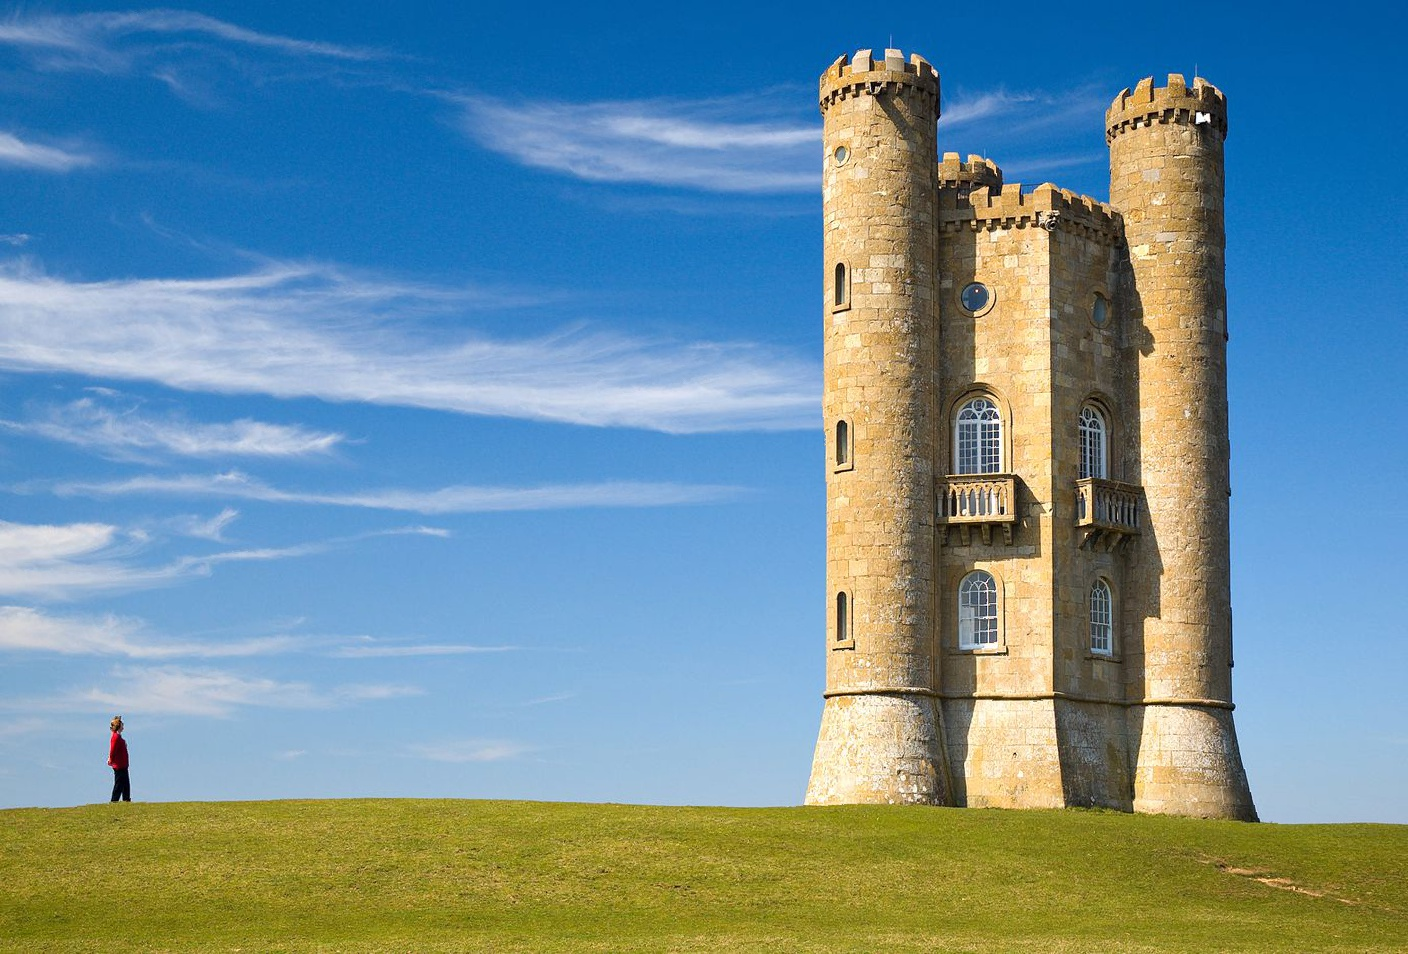
\includegraphics[scale = .3]{1Amplify.jpg}

    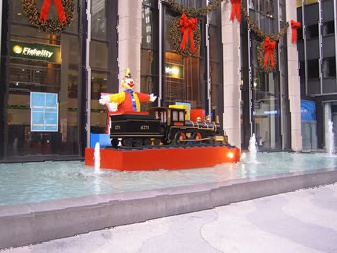
\includegraphics[scale = .3]{3Amplify.jpg}

    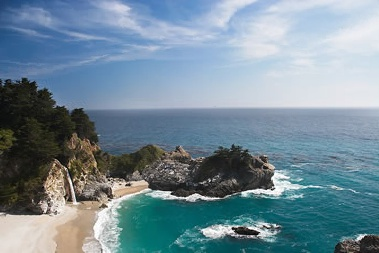
\includegraphics[scale = .3]{4Amplify.jpg}

    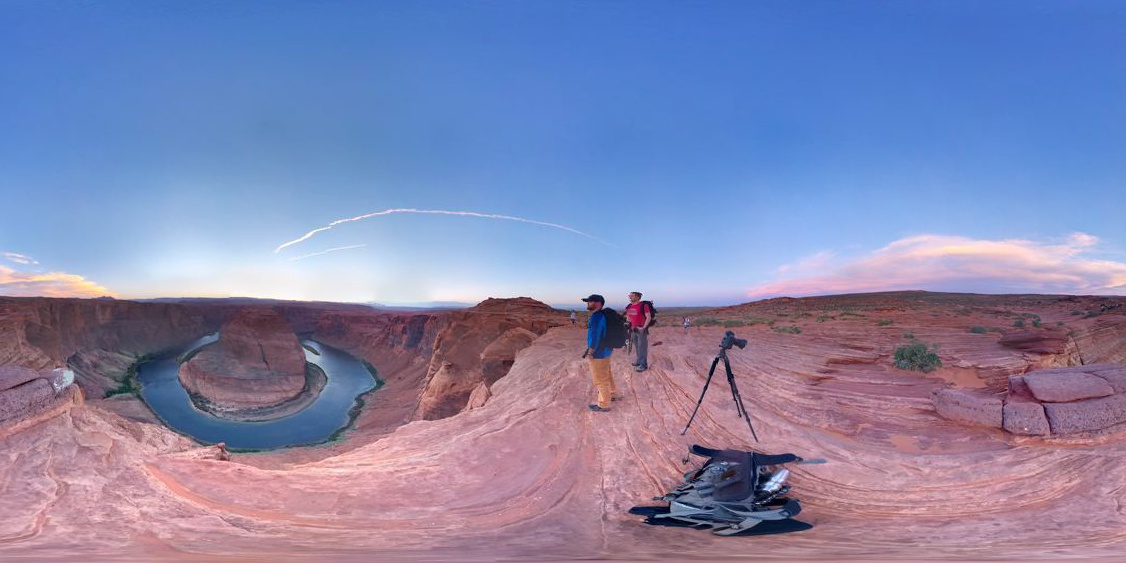
\includegraphics[scale = .3]{5Amplify.jpg}

  \section{对象移除}
    首先我们调用opencv自带的函数来选出要移除的选取,记录在maskremove里面。然后将图中这些要remove的东西的energy function中的权值置为一个很大的负权值,这样就可以在寻找seam的时候每次都删除掉remove区域里的点了。至于选择删除行还是列,这是使用的是贪心,如果行的seam值更小,就删除行。对于行列都计算一遍即可。

    \begin{lstlisting}
// 2. 创建一个可交互的窗口
    Image showImg = input.clone(); // 拷贝一张图用于显示(因为需要在显示的图上面高亮标注,从而造成修改)
    cv::namedWindow("Draw ROI", CV_WINDOW_AUTOSIZE); // 新建一个窗口
    vector<vector<int > > maskRemove(row, vector<int >(col, 0)); // 希望获取的待删除选区
    MouseArgs *args = new MouseArgs(showImg, maskRemove, Color(0, 0, 255)); // 攒一个MouseArgs结构体用于交互
    cv::setMouseCallback("Draw ROI", onMouse, (void*)args); // 给窗口设置回调函数

    // 拖动鼠标作画
    while (1)
    {
      cv::imshow("Draw ROI", args->img);
      // 按 esc 键退出绘图模式,获得选区
      if (cv::waitKey(100) == 27)
        break;
    }
    // maskRemove[200][400] = 1;
    bool** choosed = new bool*[row];
    for (int i = 0;i < row;++i)
      choosed[i] = new bool[col];
    for (int i = 0;i < row;++i)
      for (int j = 0;j < col;++j)
          choosed[i][j] = (maskRemove[i][j] == 1);
    while(1)
    {
      row = temp.rows;
      col = temp.cols;
      bool finished = true;
      for (int i = 0;i < row;++i)
        for (int j = 0;j < col;++j)
        {
          // printf("233%d %d\n",i,j);
          if (choosed[i][j]) finished = false;
        }
      if (finished) break;
      T nowpic;
      nowpic.pic = temp;
      getInfo(nowpic,choosed);
      if (nowpic.rseam < nowpic.cseam)
      {
        temp = nowpic.rowpic;
        row = temp.rows;
        col = temp.cols;
        // printf("%d %d\n",row,col);
        bool** gg = new bool*[row];
        for (int i = 0;i < row;++i)
          gg[i] = new bool[col];
        for (int i = col-1;i;--i)
          for (int j = 0,k = 0;j < row;++j)
            if (nowpic.rowseam[col-1-i].y != j)
              gg[k++][i] = choosed[j][i];
        for (int i = 0;i < row + 1;++i)
          delete[] choosed[i];
        delete[] choosed;
        choosed = gg;
      }
      else
      {
        temp = nowpic.colpic;
        row = temp.rows;
        col = temp.cols;
        // printf("%d %d\n",row,col);
        bool** gg = new bool*[row];
        for (int i = 0;i < row;++i)
          gg[i] = new bool[col];
        for (int i = row-1;i;--i)
          for (int j = 0,k = 0;j < col;++j)
            if (nowpic.colseam[row-1-i].x != j)
              gg[i][k++] = choosed[i][j];
        for (int i = 0;i < row;++i)
          delete[] choosed[i];
        delete[] choosed;
        choosed = gg;
      }
    }
    // 4. 垃圾回收
    cv::setMouseCallback("Draw ROI", NULL, NULL); // 取消回调函数
    delete args; // 垃圾回收
    // waitKey(0);

    // imshow("window",temp);
    imwrite("result.jpg",temp);
    waitKey(0);
    \end{lstlisting}

    代码流程也就像我说的一样,先获取remove区域,然后对于remove区域中的点的energy设一个负权值,然后不停地删除seam直到删完remove区域中的点。

    下面是效果:

    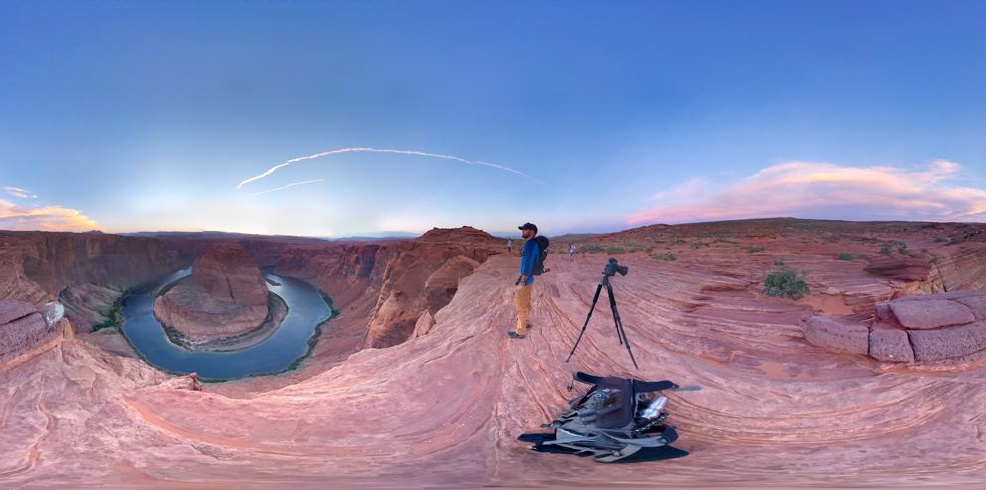
\includegraphics[scale = .1]{5remove.jpg}

    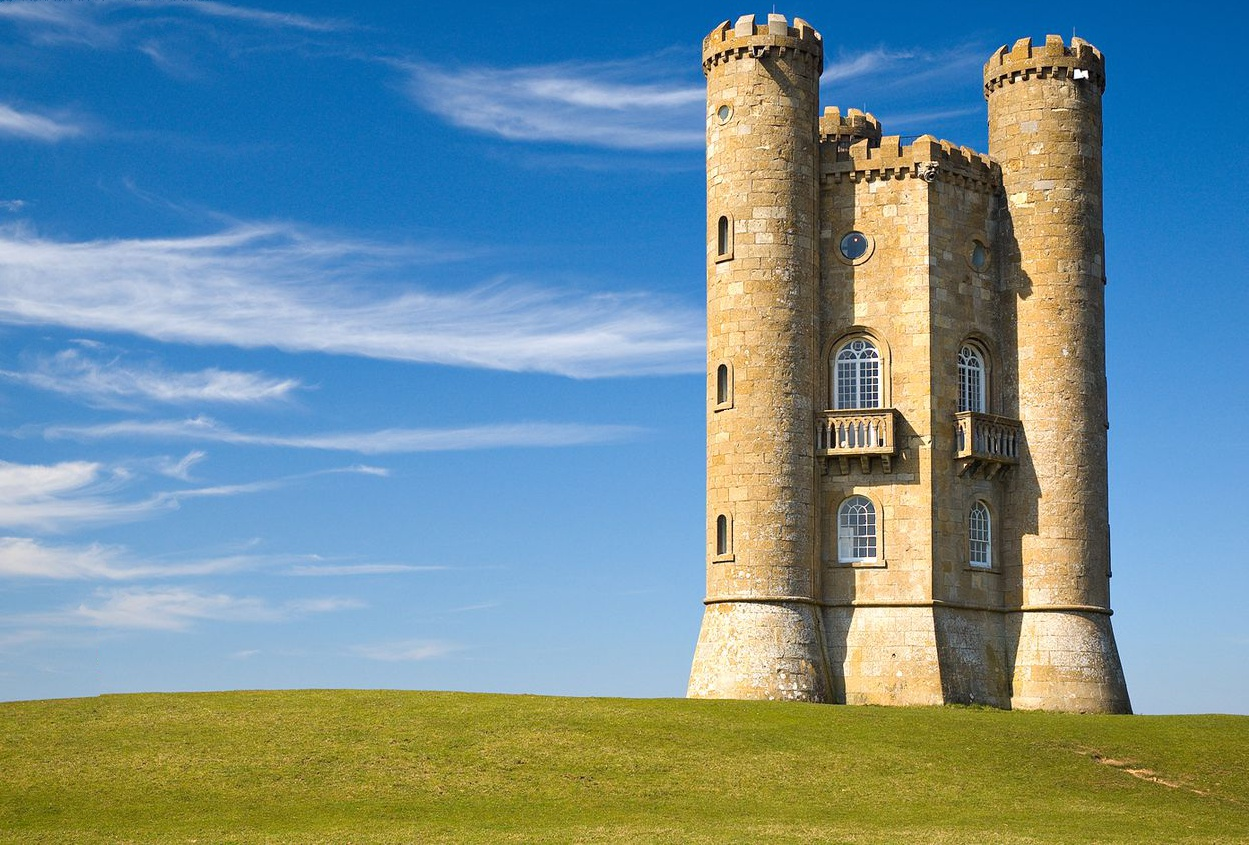
\includegraphics[scale = .2]{1remove.jpg}
  \section{自选例子}

    以下均使用Sobel算子。

    双向移除:

    原图:

    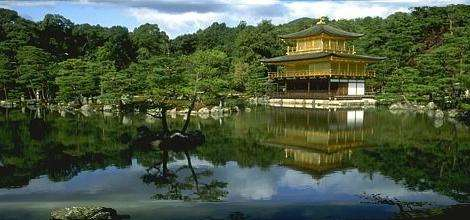
\includegraphics[scale = .3]{input.jpeg}

    
\includegraphics[scale = .3]{hhh.jpg}

    \includegraphics[scale = .3]{666.bmp}

    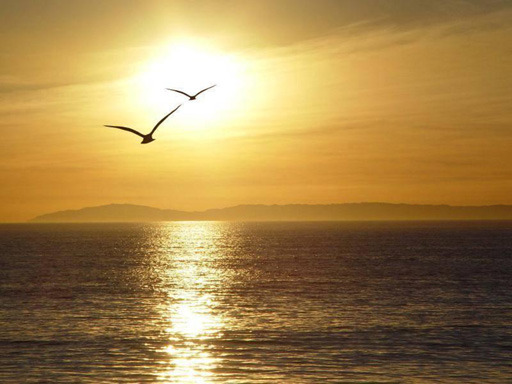
\includegraphics[scale = .3]{ori.jpg}

    双向移除后10$\%$:

    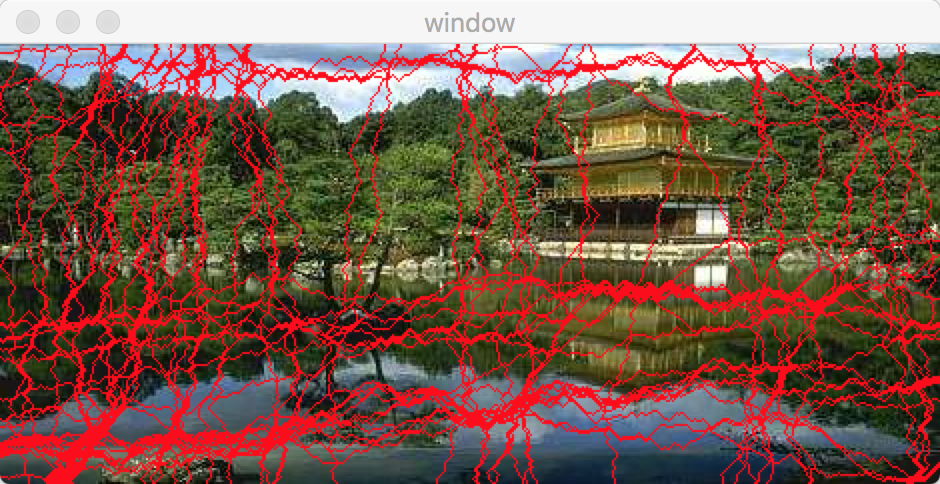
\includegraphics[scale = .3]{inputsobelseam.png}

    
\includegraphics[scale = .3]{hhhsobelseam.png}

    \includegraphics[scale = .3]{666.bmp}

    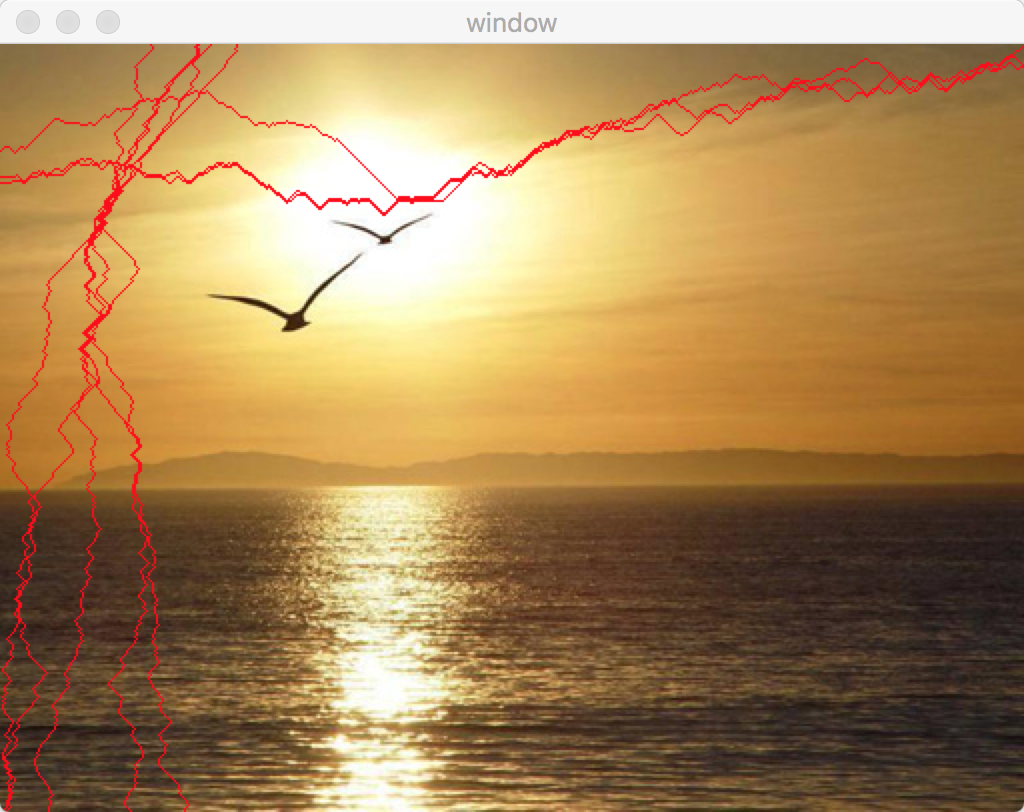
\includegraphics[scale = .3]{orisobelseam.png}

    \includegraphics[scale = .3]{inputsobel.jpg}

    
\includegraphics[scale = .3]{hhhsobel.jpg}

    
\includegraphics[scale = .3]{666sobel.jpg}

    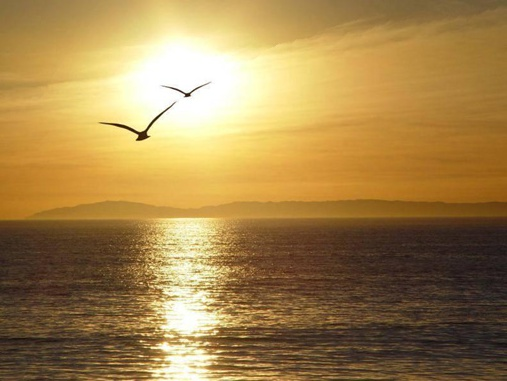
\includegraphics[scale = .3]{orisobel.jpg}

    放大:
    \includegraphics[scale = .3]{inputAmplify.jpg}

    \includegraphics[scale = .3]{hhhAmplify.jpg}

    \includegraphics[scale = .3]{666Amplify.jpg}

    \includegraphics[scale = .3]{oriAmplify.jpg}


\end{document}






































